% =====================================================================
%  TEMPLATE D'ÉTUDE — Transitions démographiques / Transitions économiques
%  Compilation : xelatex template_2026.tex (x2 pour la table des matières)
% =====================================================================
\documentclass[12pt,a4paper]{article}

% --------------------------- Polices & langue ------------------------
\usepackage{fontspec}
\setmainfont{EB Garamond}          % police du template Word d'origine
\newfontfamily\headingfont{EB Garamond}

% --------------------------- Mise en page -----------------------------
\usepackage[a4paper,top=3.25cm,bottom=2cm,left=2.5cm,right=2.5cm,headheight=28pt]{geometry}
\usepackage{xcolor}
\definecolor{brandnavy}{HTML}{243443}   % couleur exacte fournie
\definecolor{brandgrey}{HTML}{595959}

\usepackage{graphicx}
\usepackage{tikz}
\usetikzlibrary{calc}
\usepackage{eso-pic}                    % fond de page complet (couverture)
\usepackage{titlesec}
\usepackage{fancyhdr}
\usepackage{enumitem}
\usepackage{microtype} 
\hyphenpenalty=10000
\exhyphenpenalty=10000
\tolerance=9999       
\emergencystretch=3em
\usepackage[hidelinks,colorlinks=true,linkcolor=brandnavy,urlcolor=brandnavy,citecolor=brandnavy]{hyperref}
\usepackage{booktabs} 
\usepackage{multirow}
\usepackage[flushleft]{threeparttable}

% Légendes et titres en français : sans babel, LaTeX écrit « Table » et « Contents »
\renewcommand{\tablename}{Tableau}
\renewcommand{\figurename}{Figure}
\renewcommand{\contentsname}{Table des matières}

% Seuils de significativite en exposant : \sym{***}, \sym{\dag}...
\newcommand{\sym}[1]{\textsuperscript{#1}}

% La police EB Garamond "Bold" fournie par le système ne contient pas les
% caractères accentués : on retire le \bfseries par défaut des entrées de
% table des matières (article.cls) pour éviter les caractères manquants.
\usepackage{etoolbox}
\makeatletter
\patchcmd{\l@section}{\bfseries}{}{}{}
\makeatother

% Chemin du logo (image fournie par l'utilisateur)
\newcommand{\logoPath}{assets/logo.jpg}
\newcommand{\logoPathi}{assets/logo1.jpg}

% --------------------------- Titres de section -------------------------
% NB : la coupe "Bold" de la police EB Garamond fournie par Ubuntu ne contient
% pas les caractères accentués. On évite donc le gras et on distingue les
% titres par la couleur, la taille et l'approche des capitales.
\titleformat{\section}
{\headingfont\color{brandnavy}\Large}
{\thesection.}{0.6em}{}
\titlespacing*{\section}{0pt}{2.4em}{1.2em}

\titleformat{\subsection}
{\headingfont\color{brandnavy}\large\itshape}
{\thesubsection.}{0.6em}{}
\titlespacing*{\subsection}{0pt}{1.6em}{0.8em}

% --------------------------- En-tête / pied de page ---------------------
\pagestyle{fancy}
\fancyhf{}
\renewcommand{\headrulewidth}{0.4pt}
\renewcommand{\footrulewidth}{0pt}
\fancyhead[L]{\footnotesize\color{brandgrey}\itshape\leftmark}
\fancyhead[R]{\raisebox{-0.2\height}{\includegraphics[height=1cm]{\logoPathi}}}
\fancyfoot[C]{\footnotesize\color{brandgrey}\thepage}
\renewcommand{\sectionmark}[1]{\markboth{#1}{}}

\fancypagestyle{plain}{%
	\fancyhf{}
	\fancyfoot[C]{\footnotesize\color{brandgrey}\thepage}
	\renewcommand{\headrulewidth}{0pt}
}

% =====================================================================
%                        VARIABLES DU DOCUMENT
%  -> à modifier pour chaque nouvelle étude
% =====================================================================
\newcommand{\etudeTitre}{Logement et politique familiale}
\newcommand{\etudeSousTitre}{Quelles conséquences sur la natalité ?}
\newcommand{\etudeAuteur}{GENNA Kévin}
\newcommand{\etudeDate}{Septembre 2026} % pas de \today : sans babel, il s'affiche en anglais — indiquez la date à la main

\definecolor{srcv1}{HTML}{1F4E79}
\definecolor{srcv2}{HTML}{B9770E}
\definecolor{srcv3}{HTML}{C0392B}
\definecolor{srcvE}{HTML}{707070}

\begin{document}
	
	% =====================================================================
	% PAGE DE COUVERTURE
	% =====================================================================
	\begin{titlepage}
		\AddToShipoutPicture*{%
			\put(0,0){%
				\begin{tikzpicture}[remember picture,overlay]
					\fill[brandnavy] (current page.south west) rectangle (current page.north east);
				\end{tikzpicture}%
			}%
		}
		\thispagestyle{empty}
		\color{white}
		\begin{center}
			\vspace*{-3cm}
			\includegraphics[width=0.6\textwidth]{\logoPath}\\[2.8cm]
			{\headingfont\fontsize{36}{42}\selectfont \etudeTitre}\\[0.8cm]
			{\headingfont\Large\itshape \etudeSousTitre}\\[2.5cm]
			\vfill
			{\headingfont\Large \etudeAuteur \\ 
				\quad \\
				\etudeDate}
			\vspace*{6.5cm}
		\end{center}
	\end{titlepage}
	
	\color{black}
	
	% =====================================================================
	% RÉSUMÉ
	% =====================================================================
	\section*{Résumé}
	\addcontentsline{toc}{section}{Résumé}
	\markboth{Résumé}{}
	
	Longtemps l'exception européenne, la fécondité française recule depuis 2012 et l'indicateur conjoncturel de fécondité est tombé à 1,56 enfant par femme en 2025. Cette étude interroge deux des explications les plus souvent avancées, le logement et la politique familiale, à partir des huit vagues 2006-2025 de l'enquête Statistiques sur les ressources et conditions de vie (SRCV) de l'Insee, en replaçant le couple et sa décision d'avoir un enfant au centre de l'analyse. \\

\noindent Sur le logement, quatre constats. Les jeunes ménages locataires ont surtout perdu de l'espace : à taux d'effort stable, leur surface a reculé de deux à huit mètres carrés selon l'âge entre 2006 et 2025, pendant que les accédants voyaient leur taux d'effort baisser de huit points grâce à la chute des taux d'intérêt. Ensuite, ce qui compte pour la natalité n'est pas le prix du logement mais ce qu'il permet d'occuper : à prix au mètre carré, revenu et âge donnés, le coût n'a aucun effet, la surface en a un, concentré sur le premier enfant, et il prend la forme d'une marche plutôt que d'une pente. Un couple sans enfant logé dans moins de 60 mètres carrés a une probabilité de première naissance inférieure de huit à dix points à celle d'un couple logé dans 70 à 89 mètres carrés, sur un taux de référence de 14,5\,\% ; au-dessus, la surface ne départage plus rien. Troisièmement, cette association est solide mais elle n'est probablement pas causale : elle survit chez les ménages installés depuis trois ans ou plus et elle est plus forte là où le marché est tendu, mais, sur les mêmes ménages, la surface est liée à la naissance récente et ne prédit pas la naissance suivante, ce qui ressemble davantage à un logement choisi pour un projet de famille qu'à une contrainte. Enfin, l'avantage des accédants sur les locataires pour le premier enfant, de cinq à sept points à âge et revenu égaux, n'est ni un effet d'âge, ni un effet de revenu, ni un effet de patrimoine ; il tient pour un quart à la surface et pour le reste à ce que le statut porte en propre, sans que l'on puisse exclure qu'il soit lui-même le signe d'une installation déjà décidée. \\

\noindent La question centrale, la part de la baisse de la fécondité depuis 2010 que le logement peut porter, reçoit une réponse en deux temps. Le canal de la surface, lu en tranches, reproduirait entre un vingtième et un dixième de la baisse selon la borne retenue, parce que la part des couples sans enfant logés dans un petit logement a augmenté pendant que la surface moyenne ne bougeait pas. Mais la progression de l'accession à la propriété, portée par les taux bas, a joué en sens inverse d'un montant comparable, de sorte que le solde du logement est indiscernable de zéro. Ce solde nul repose entièrement sur le canal de l'accession, le plus exposé à la causalité inverse ; sans lui, le logement porterait au plus un dixième de la baisse. Ces ordres de grandeur supposent de transposer aux femmes dans leur ensemble ce que nous mesurons sur les couples constitués, et ils résistent aux fragilités de mesure des vagues récentes. La hausse du niveau de vie pèse davantage, et le vieillissement du champ fécond moins qu'on ne l'écrit souvent, sans qu'aucun des deux ne relève du logement. \\

\noindent Sur la politique familiale, les prestations en espèces croissent avec le rang mais leur poids dans le revenu des familles nombreuses a été divisé par près de deux en vingt ans, de 21,5 à 13,2\,\% pour une troisième naissance ; le quotient familial, à l'inverse, ne procure aucun avantage à 86\,\% des ménages du premier quintile et près de 2\,000 euros par an à ceux du dernier. Enfin, parmi les mères d'un enfant de moins de trois ans, le maintien en emploi, congé de maternité compris, se joue d'abord sur le diplôme, marqueur du coût d'opportunité d'une interruption, bien plus que sur l'âge de l'enfant ; l'écart selon le statut de logement, considérable, relève pour l'essentiel de la sélection. Une politique familiale qui privilégie l'avantage fiscal au service en nature aide, par construction, les ménages qui en ont le moins besoin pour travailler.
	
	\newpage
	
	% =====================================================================
	% TABLE DES MATIÈRES
	% =====================================================================
	\tableofcontents
	\thispagestyle{plain}
	\newpage
	
	% =====================================================================
	% CORPS DE L'ÉTUDE
	% =====================================================================
	\section{Introduction}
	
Longtemps vue comme une exception, la forte natalité française commence elle aussi à fléchir, et se retrouve plus proche que jamais de nos voisins européens. L’indicateur conjoncturel de fécondité est descendu à 1,56 enfant par femme en 2025, son niveau le plus faible depuis la fin de la Première Guerre mondiale (Insee, 2026). Pire encore, pour la première fois sur une année, le nombre de décès a excédé le nombre de naissances, à la faveur d’une pyramide démographique fortement déformée par la nombreuse génération des baby-boomers, et d’une natalité qui se contracte d’années en années depuis 2012. \\

\noindent Bien que les dynamiques démographiques soient difficiles à anticiper, une tendance claire semble se dessiner à travers le monde, et en particulier dans les pays de l’OCDE (hors Israël). La natalité faiblit, du cas extrême de la Corée du Sud avec une fécondité sous les 0,8 enfants par femme à la Suède (1,5), l’Italie (1,2) et même jusqu’aux Etats-Unis (1,4), les pays membres de l’OCDE sont loin du taux de renouvellement des générations de 2,05 enfants par femme. De nombreuses études\footnote{Doepke et al. (2023) ; Couillard (2025) ; Saudubray (2026).} tentent de décrypter pourquoi la fécondité baisse : logement, politiques familiales, inégalités hommes femmes persistantes, fin des structures de couple classique, manque de confiance en l’avenir … Il s’avère alors que la chute de la natalité est multiforme et ne puisse se traiter de manière holistique par un seul canal. Le récent rapport de l’assemblée nationale sur la mission d’information liée aux causes et aux conséquences de la baisse de la natalité\footnote{Assemblée nationale (2026), rapport d’information n\textsuperscript{o} 2474 de la mission d’information sur les causes et conséquences de la baisse de la natalité en France, déposé le 11 février 2026 (présidente C. de Pélichy, rapporteur J. Patrier-Leitus).} ne s’y est pas trompé, de nouvelles solutions sont à mettre en place et plusieurs points sont à analyser avec finesse, notamment le rôle du logement mais aussi celui des politiques familiales. \\

\noindent Dans cette étude nous remettons le couple et sa décision d’avoir un enfant au cœur du processus de procréation, avec une emphase plus particulière sur le cas de la France. Les enjeux que nous voulons traiter ici sont les facteurs influençant directement le couple mais indirectement la fécondité : le logement, la politique familiale et les choix de garde d’enfant. Le premier objet semble essentiel à nos yeux, car depuis les années 2000, un couple aux revenus médian a perdu près de 20m$^2$ de capacité d’achat\footnote{Meilleurs agents (2022)}  soit l’équivalent d’une seconde voire d’une troisième chambre dans un logement. Aux États-Unis, Couillard (2025) impute à la hausse du coût du logement depuis 1990 une part importante du recul des naissances : à coût du logement inchangé, treize millions d’enfants supplémentaires seraient nés entre 1990 et 2020. Le cas des politiques familiales semble plus complexe à analyser, car la France est encore le 5$^e$ pays de l’OCDE sur les dépenses de politique familiale en points de PIB, mais elle se différencie des pays scandinaves avec des exonérations d’impôts qui comptent pour près d’un quart des dépenses familiales (contre 0 dans les pays du Nord). Nous discuterons comment cette conception de la politique familiale peut avoir un impact sur l’offre de travail des mères et donc aussi sur les choix de garde d’enfants. \\

\noindent L’analyse que nous proposons est une analyse purement économique et se soustrait à toute conception sociale ou sociétal de la décision d’avoir un enfant. Loin de vouloir négliger cet aspect, qui revêt un attrait plus sociologique voire idéologique (comme le mouvement « No Kids », même s’il reste relativement marginal\footnote{Selon l’Ined, la part des personnes ne souhaitant pas d’enfant est de l’ordre de 5\,\% (4,4\,\% des femmes, 6,8\,\% des hommes) et n’a pas augmenté depuis 1995 (Debest et Mazuy, 2014).}), nous préférons apposer la focale sur les mécanismes économiques de la fertilité. La première raison est que nous sommes une équipe d’économistes donc nous nous concentrons sur notre cœur de métier, la seconde est que le sujet est extrêmement large et que nous ne pouvons avoir l’ambition de traiter tous ces sujets en une seule étude, il nous faut donc concentrer notre analyse. \\

\noindent Pour mener à bien cette étude nous allons utiliser les Statistiques sur les Ressources et Conditions de Vie (SRCV) éditées chaque année par l’Insee. Il s’agit de données individuelles et représentatives des ménages français, avec des informations sur les naissances au sein des ménages, le niveau de vie, la taille du logement, est-ce que le ménage est propriétaire ou locataire, la part des prestations familiales dans le revenu disponible … Cette source nous permet de traiter les effets du logement mais aussi des prestations familiales en espèces, parmi d’autres variables, sur la probabilité qu’une naissance ait lieu. Nous mobilisons huit vagues de cette enquête, 2006, 2010, 2014 et 2018, puis chacune des années 2022 à 2025, soit près de vingt ans de conditions de logement mesurées de façon homogène. Les modèles de la partie 3 les empilent toutes, avec des effets fixes d’année, ce qui donne à l’analyse des naissances une puissance qu’une seule vague ne pourrait offrir ; les évolutions de long terme sont lues entre 2006 ou 2010 et 2025. Les vagues 2022 à 2025, seules à documenter l’activité au niveau individuel, servent seules à la partie 4 sur l’emploi des mères. 
	
	\section{Se loger en France}
	
Un des points qui revient le plus souvent lorsque l’on parle de la baisse de la fécondité est le logement, et cela se comprend car pour avoir un enfant il faut pouvoir l’héberger dans des conditions décentes. Ainsi la décision de procréer peut d’abord passer par la location ou l’acquisition d’un logement adéquat. \\

\noindent Dans cette partie nous nous intéresserons à l’évolution du logement, son prix, sa surface, sa disponibilité pour établir une cartographie des logements de 2006 à 2025. Pour ce faire nous utiliserons les données SRCV qui suivent plusieurs milliers de ménages chaque année, et qui vont nous permettre de dresser un bilan précis des conditions de logements des ménages français. 

\subsection{L'évolution des ménages et de leur logement}

Les données utilisées nous permettent d'avoir une vue sur quasiment 20 ans de l'évolution des ménages et de leur logement, et la richesses de l'information nous donne une idée de la composition des ménages. Nous proposons d'abord une description statistique des données que nous utilisons entre 2014 et 2025, avec un point d'étape en 2018\footnote{Nous ne pouvons pas remonter jusqu'à 2006 ici car les données avant 2014 diffèrent et certaines informations, comme la tranche d'unité urbaine, ne sont disponibles qu'à partir de 2014}. Il s'agit pour nous de présenter la moyenne de l'âge des ménage, le nombre de naissances pour 1000 ménages, les ressources, les caractéristiques moyennes des logement et son coût.  

\begin{table}[h!]
	\centering
	\small
	\setlength{\tabcolsep}{2pt}
	\begin{threeparttable}
		\caption{Caractéristiques des ménages comportant une femme de 15 à 49 ans, selon le statut d'occupation : \textcolor{srcv1}{2014}\,\textbar\,\textcolor{srcv2}{2018}\,\textbar\,\textcolor{srcv3}{2025}}
		\label{tab:descriptif_statut}
		\begin{tabular}{l@{\hspace{5pt}}r@{\,\textbar\,}r@{\,\textbar\,}r@{\hspace{7pt}}r@{\,\textbar\,}r@{\,\textbar\,}r@{\hspace{7pt}}r@{\,\textbar\,}r@{\,\textbar\,}r}
			\toprule
			& \multicolumn{3}{c}{Locataires} & \multicolumn{3}{c}{Accédants} & \multicolumn{3}{c}{Non accédants} \\
			\cmidrule(lr){2-4}     \cmidrule(lr){5-7}     \cmidrule(lr){8-10}
			& \textcolor{srcv1}{2014} & \textcolor{srcv2}{2018} & \textcolor{srcv3}{2025} & \textcolor{srcv1}{2014} & \textcolor{srcv2}{2018} & \textcolor{srcv3}{2025} & \textcolor{srcv1}{2014} & \textcolor{srcv2}{2018} & \textcolor{srcv3}{2025} \\
			\midrule
			\multicolumn{10}{l}{\textit{Démographie}} \\
			Âge moyen des parents (ans) & \textcolor{srcv1}{35,3} & \textcolor{srcv2}{35,2} & \textcolor{srcv3}{35,6} & \textcolor{srcv1}{38,9} & \textcolor{srcv2}{39,1} & \textcolor{srcv3}{38,9} & \textcolor{srcv1}{42,2} & \textcolor{srcv2}{44,3} & \textcolor{srcv3}{40,5} \\
			Taille du ménage (avant naiss.) & \textcolor{srcv1}{2,57} & \textcolor{srcv2}{2,67} & \textcolor{srcv3}{2,76} & \textcolor{srcv1}{3,42} & \textcolor{srcv2}{3,40} & \textcolor{srcv3}{3,24} & \textcolor{srcv1}{3,18} & \textcolor{srcv2}{3,42} & \textcolor{srcv3}{3,08} \\
			Familles monoparentales (\%) & \textcolor{srcv1}{18,9} & \textcolor{srcv2}{17,7} & \textcolor{srcv3}{21,5} & \textcolor{srcv1}{5,4} & \textcolor{srcv2}{5,2} & \textcolor{srcv3}{4,8} & \textcolor{srcv1}{6,2} & \textcolor{srcv2}{7,6} & \textcolor{srcv3}{11,8} \\
			Naissances pour 1\,000 ménages & \textcolor{srcv1}{98} & \textcolor{srcv2}{83} & \textcolor{srcv3}{48} & \textcolor{srcv1}{95} & \textcolor{srcv2}{93} & \textcolor{srcv3}{70} & \textcolor{srcv1}{44} & \textcolor{srcv2}{31} & \textcolor{srcv3}{32} \\
			\addlinespace
			\multicolumn{10}{l}{\textit{Ressources}} \\
			Revenu disponible (k\texteuro/an) & \textcolor{srcv1}{36,7} & \textcolor{srcv2}{38,9} & \textcolor{srcv3}{40,6} & \textcolor{srcv1}{61,6} & \textcolor{srcv2}{64,1} & \textcolor{srcv3}{69,2} & \textcolor{srcv1}{60,6} & \textcolor{srcv2}{67,2} & \textcolor{srcv3}{59,6} \\
			Niveau de vie (k\texteuro/an/UC) & \textcolor{srcv1}{22,1} & \textcolor{srcv2}{23,4} & \textcolor{srcv3}{24,1} & \textcolor{srcv1}{31,0} & \textcolor{srcv2}{32,3} & \textcolor{srcv3}{36,1} & \textcolor{srcv1}{30,3} & \textcolor{srcv2}{32,1} & \textcolor{srcv3}{30,5} \\
			\addlinespace
			\multicolumn{10}{l}{\textit{Logement}} \\
			Surface du logement (m\textsuperscript{2}) & \textcolor{srcv1}{71,7} & \textcolor{srcv2}{70,6} & \textcolor{srcv3}{68,7} & \textcolor{srcv1}{112,1} & \textcolor{srcv2}{111,0} & \textcolor{srcv3}{112,4} & \textcolor{srcv1}{111,1} & \textcolor{srcv2}{112,8} & \textcolor{srcv3}{107,7} \\
			Nombre de pièces & \textcolor{srcv1}{3,25} & \textcolor{srcv2}{3,29} & \textcolor{srcv3}{3,21} & \textcolor{srcv1}{4,67} & \textcolor{srcv2}{4,65} & \textcolor{srcv3}{4,58} & \textcolor{srcv1}{4,61} & \textcolor{srcv2}{4,69} & \textcolor{srcv3}{4,54} \\
			Surface par personne (m\textsuperscript{2}) & \textcolor{srcv1}{32,7} & \textcolor{srcv2}{31,2} & \textcolor{srcv3}{30,4} & \textcolor{srcv1}{36,1} & \textcolor{srcv2}{36,2} & \textcolor{srcv3}{38,4} & \textcolor{srcv1}{39,0} & \textcolor{srcv2}{36,0} & \textcolor{srcv3}{40,9} \\
			Surface par pièce (m\textsuperscript{2}) & \textcolor{srcv1}{22,9} & \textcolor{srcv2}{22,2} & \textcolor{srcv3}{22,0} & \textcolor{srcv1}{24,3} & \textcolor{srcv2}{24,1} & \textcolor{srcv3}{24,8} & \textcolor{srcv1}{24,6} & \textcolor{srcv2}{25,2} & \textcolor{srcv3}{24,1} \\
			\addlinespace
			\multicolumn{10}{l}{\textit{Coût}} \\
			Coût du logement (\texteuro/mois) & \textcolor{srcv1}{867} & \textcolor{srcv2}{837} & \textcolor{srcv3}{885} & \textcolor{srcv1}{1\,715} & \textcolor{srcv2}{1\,644} & \textcolor{srcv3}{1\,703} & \textcolor{srcv1}{316} & \textcolor{srcv2}{349} & \textcolor{srcv3}{294} \\
			Coût au m\textsuperscript{2} (\texteuro/mois) & \textcolor{srcv1}{13,56} & \textcolor{srcv2}{13,45} & \textcolor{srcv3}{14,49} & \textcolor{srcv1}{16,69} & \textcolor{srcv2}{16,50} & \textcolor{srcv3}{17,89} & \textcolor{srcv1}{3,12} & \textcolor{srcv2}{3,38} & \textcolor{srcv3}{3,24} \\
			Taux d'effort (\%) & \textcolor{srcv1}{34,0} & \textcolor{srcv2}{31,6} & \textcolor{srcv3}{32,4} & \textcolor{srcv1}{36,6} & \textcolor{srcv2}{34,2} & \textcolor{srcv3}{31,2} & \textcolor{srcv1}{8,0} & \textcolor{srcv2}{8,3} & \textcolor{srcv3}{8,4} \\
			\addlinespace
			\multicolumn{10}{l}{\textit{Géographie}} \\
			Rural (\%) & \textcolor{srcv1}{13,9} & \textcolor{srcv2}{11,9} & \textcolor{srcv3}{10,7} & \textcolor{srcv1}{29,9} & \textcolor{srcv2}{26,7} & \textcolor{srcv3}{27,0} & \textcolor{srcv1}{29,9} & \textcolor{srcv2}{32,5} & \textcolor{srcv3}{27,8} \\
			Unité urbaine < 20\,000 hab. (\%) & \textcolor{srcv1}{14,7} & \textcolor{srcv2}{13,5} & \textcolor{srcv3}{12,1} & \textcolor{srcv1}{20,2} & \textcolor{srcv2}{19,2} & \textcolor{srcv3}{20,2} & \textcolor{srcv1}{17,4} & \textcolor{srcv2}{21,5} & \textcolor{srcv3}{20,9} \\
			20\,000 à 199\,999 hab. (\%) & \textcolor{srcv1}{22,7} & \textcolor{srcv2}{21,9} & \textcolor{srcv3}{19,2} & \textcolor{srcv1}{15,2} & \textcolor{srcv2}{15,6} & \textcolor{srcv3}{16,4} & \textcolor{srcv1}{16,5} & \textcolor{srcv2}{10,1} & \textcolor{srcv3}{15,9} \\
			200\,000 hab. à 2 M (\%) & \textcolor{srcv1}{33,7} & \textcolor{srcv2}{31,0} & \textcolor{srcv3}{34,9} & \textcolor{srcv1}{20,6} & \textcolor{srcv2}{23,3} & \textcolor{srcv3}{22,9} & \textcolor{srcv1}{18,8} & \textcolor{srcv2}{20,1} & \textcolor{srcv3}{20,3} \\
			Agglomération de Paris (\%) & \textcolor{srcv1}{15,1} & \textcolor{srcv2}{21,7} & \textcolor{srcv3}{23,1} & \textcolor{srcv1}{14,1} & \textcolor{srcv2}{15,2} & \textcolor{srcv3}{13,5} & \textcolor{srcv1}{17,5} & \textcolor{srcv2}{15,9} & \textcolor{srcv3}{15,1} \\
			\addlinespace
			\midrule
			Part dans le champ (\%) & \textcolor{srcv1}{43,8} & \textcolor{srcv2}{45,9} & \textcolor{srcv3}{48,0} & \textcolor{srcv1}{44,1} & \textcolor{srcv2}{46,0} & \textcolor{srcv3}{42,0} & \textcolor{srcv1}{12,1} & \textcolor{srcv2}{8,1} & \textcolor{srcv3}{10,0} \\
			Effectif (non pondéré) & \textcolor{srcv1}{1\,632} & \textcolor{srcv2}{1\,493} & \textcolor{srcv3}{1\,847} & \textcolor{srcv1}{1\,969} & \textcolor{srcv2}{1\,701} & \textcolor{srcv3}{2\,303} & \textcolor{srcv1}{551} & \textcolor{srcv2}{356} & \textcolor{srcv3}{541} \\
			\bottomrule
		\end{tabular}
		\begin{tablenotes}[flushleft]\scriptsize
			\item \textit{Lecture} : chaque case donne les moyennes pondérées de \textcolor{srcv1}{2014}\,\textbar\,\textcolor{srcv2}{2018}\,\textbar\,\textcolor{srcv3}{2025}.
			\item \textit{Statuts} : \textit{Accédants} = propriétaires remboursant un emprunt sur
			leur résidence principale ; \textit{Non accédants} = propriétaires sans emprunt en cours.
			\item \textit{Champ} : ménages comportant une femme de 15 à 49      ans (personne de référence ou conjointe), France entière --- couples et familles
			monoparentales. Les familles monoparentales dirigées par un homme en sont absentes
			par construction : la part reportée est celle des mères isolées.
			\item \textit{Âge moyen du ou des parents} : moyenne d'âge de la personne de référence
			et de son conjoint, \textbf{enfants exclus} (fichier individus). Pour une famille
			monoparentale, c'est l'âge du parent seul.
			\item \textit{Familles monoparentales} : ménages hors couple ayant au moins un enfant.
			\item \textit{Géographie} : tranche d'unité urbaine de la commune de résidence, regroupée
			en cinq classes ; les cinq parts somment à 100\,\% dans chaque colonne. Source :
			\texttt{tuu10} (2014, 2018, population 2010) puis \texttt{TUU2017} (2025, population
			2017) --- même concept, seule l'année de référence du recensement change.
			Le degré d'urbanisation \texttt{DB100} n'est pas utilisé : la nomenclature Eurostat
			DEGURBA a été révisée vers 2011-2012 et ses niveaux ne sont pas comparables entre
			vagues. Les millésimes antérieurs à 2014 ne portent que \texttt{TAU99}, qui mesure des
			\textit{aires} urbaines et non des \textit{unités} urbaines.
			\item \textit{Montants} : euros constants 2025 (IPC Insee) ; k\texteuro{} = milliers d'euros.
			Coût du logement =
			charges (\texttt{HH070}) + mensualité de remboursement (\texttt{REMP}/\texttt{REMPR}).
			Taux d'effort = coût annuel rapporté au revenu disponible, borné à [0 ; 100]\,\%.
			\item \textit{Naissances} : ménages déclarant une naissance récente, pour 1\,000
			ménages du statut. \textbf{Attention} : la naissance est mesurée par \texttt{EVENEMEN\_C}
			(naissance dans l'année) jusqu'en 2018 et reconstruite depuis le fichier individus
			(enfant né en N ou N-1) à partir de 2022. L'écart franchissant cette rupture mélange
			évolution réelle et changement de mesure ; les sous-périodes situées d'un même côté
			de 2018 sont, elles, comparables.
			\item \textit{Millésimes} : 2023 et 2024 sont exclus (anomalie de pondération
			documentée dans R/17--18).
			\item \textit{Source} : Insee, SRCV 2014, 2018, 2025, calculs de l'auteur.
		\end{tablenotes}
	\end{threeparttable}
\end{table}




\newpage

\subsection{Augmentation des prix et baisse des surfaces, les jeunes ménages pris en tenaille}

L’intérêt pour nous est de regarder l’évolution des prix et des surfaces pour les ménages les plus jeunes, car ce sont eux qui sont en mesure d’avoir des enfants. Nous nous intéresserons tout particulièrement aux tranches d’âge de 20 à 40 ans, les naissances avant 20 ans ou après 40 ans restant marginales, la question du logement paraît moins pertinente. La première question est de savoir si les ménages ont vu la taille de leur logement augmenter ou diminuer sur les 20 dernières années et si leur prix a augmenté en même temps. Nous allons répondre à cette question en différenciant les locataires des propriétaires accédants\footnote{Nous faisons le choix de ne pas prendre en compte les propriétaires qui ont déjà payé leur logement, qui sont logés à titre gratuit ou qui ont hérité d’un bien.}, et nous présenterons la surface moyenne, le prix moyen du logement ainsi que le prix moyen au m² auxquels font face les locataires et les propriétaires (pour les propriétaires la totalité de la charge est égale aux frais de copropriété plus les mensualités de remboursement d’emprunt). Nous différencions 4 grandes tranches d’âge : 20-24 ans, 25-29 ans, 30-34 ans et 35-39 ans. \\

\noindent L’intégralité des tableaux et des résultats sont disponibles en annexe \ref{annexe1}, ce qu’il faut retenir majoritairement c’est que globalement les ménages locataires de 20 à 40 ans ont vu la taille de leur logement diminuer et le prix des loyers\footnote{Déflaté de l'indice des prix à la consommation}  augmenter, -5m$^2$ et + 75€/mois pour les 20-24ans, -2m$^2$ et +50€ pour les 25-29ans, -8m$^2$ et +85€/mois pour les 30-34ans et -7m$^2$ et +83€/mois pour les 35-39ans entre 2006 et 2025. Pour les ménages accédant, la surface est resté globalement stable et le prix par mois a légèrement diminué, à la faveur de taux d’intérêt très bas entre 2012 et 2022. Ces chiffres bruts ne prennent pas en compte l'évolution des revenus des ménages, uniquement celle des prix. Dans l'annexe \ref{annexe1b} nous prenons en compte l'évolution des revenus pour caractériser l'évolution du taux d'effort des ménages de 2006 à 2025. Nos résultats montrent que chez les locataires le taux d'effort est globalement stable alors que pour les propriétaires il a progressivement diminué, -7 points pour les 25-29 ans, -4 points pour les 30-34 ans et -8 points pour les 35-39 ans\footnote{Il n'y a pas assez d'observations de propriétaires accédant chez les 20-24 ans pour produire cette statistique dans ce groupe d'âge}. Cette baisse chez les propriétaires accédant est majoritairement dû à une baisse rapide des taux d'intérêt après les crise des subprimes de 2008 et celle des dettes souveraines après 2012, où les taux d'intérêt sont restés très proches de 0 pendant de nombreuses années, réduisant ainsi le coût du crédit. Le tableau \ref{tab:logsum} ci-dessous reprend les évolutions des conditions de logement chez les 20-39 ans entre 2006 et 2025.  

\bigskip

	\begin{table}[htbp]
	\centering
	\footnotesize
	\setlength{\tabcolsep}{4pt}
	\begin{threeparttable}
		\caption{Évolution des conditions de logement chez les 20-39 ans entre 2006 et 2025 (coûts en euros constants de 2025)}
		\label{tab:logsum}
		\begin{tabular}{lrrrrrr}
			\toprule
			& \multicolumn{3}{c}{Locataires} & \multicolumn{3}{c}{Propriétaires accédants} \\
			\cmidrule(lr){2-4} \cmidrule(lr){5-7}
			Âge & \multicolumn{1}{c}{\shortstack{Surface\\(m\textsuperscript{2})}} & \multicolumn{1}{c}{\shortstack{Coût\\(\texteuro/mois)}} & \multicolumn{1}{c}{\shortstack{Effort\\(\%)}} &  \multicolumn{1}{c}{\shortstack{Surface\\(m\textsuperscript{2})}} & \multicolumn{1}{c}{\shortstack{Coût\\(\texteuro/mois)}} & \multicolumn{1}{c}{\shortstack{Effort\\(\%)}}  \\
			\midrule
			20-24 ans & -4,9 & +75 & +2,7  & --- & --- & ---  \\
			25-29 ans & -1,9 & +54 & -2,2  & +6,1 & -92 & -7,4  \\
			30-34 ans & -8,4 & +85 & -0,3  & -1,8 & -177 & -7,8  \\
			35-39 ans & -6,9 & +82 & -1,9  & -1,6 & +15 & -8  \\
			\bottomrule
		\end{tabular}
		\begin{tablenotes}[flushleft]\scriptsize
			\item \textit{Champ} : ménages dont la personne de référence a 20-39 ans, France entière.
			\item \textit{Lecture} : moyennes pondérées (poids de sondage SRCV). Coût du logement =
			charges (\texttt{HH070}) + mensualité de remboursement (\texttt{REMP}/\texttt{REMPR}).
			\item \textit{Déflateur} : coûts déflatés par l'indice des prix à la consommation (Insee, base 100 = 2025) ; les montants sont en euros de pouvoir d'achat constant.
			\item \textit{n} : effectif non pondéré de la cellule. Les moyennes reposant sur
			moins de 30 observations ne sont pas reportées et sont remplacées par ---.
			\item \textit{Source} : Insee, SRCV 2006-2025, calculs de l'auteur.
		\end{tablenotes}
	\end{threeparttable}
\end{table} 

\bigskip

\noindent En conclusion, on observe une tendance à la baisse des surfaces chez les locataires, qui s'associe à une hausse du coût à un rythme similaire aux revenus car le taux d'effort est globalement stable chez les 20-39 ans. Pour un poids similaire dans les revenus, les jeunes ménages locataires ont vu leur surface d'habitation se déprécier alors que chez les propriétaires accédant, la donne est inversée car la surface achetée est restée globalement stable mais leur taux d'effort s'est considérablement rétracté (environ 8 points de pourcentage en moins). Par la suite, nous allons tester si ces résultats sont différenciés selon les catégorie de revenus et finalement si le logement joue sur la natalité. Rappelons que Dettling et Kearney (2014) montrent, aux États-Unis, qu'une hausse des prix immobiliers relève la fécondité des propriétaires et abaisse celle des locataires ; au regard de nos résultats, on pourrait s'attendre au même type de contraste ici.  

\subsection{Des effets différenciés pour les classes de revenus}

Nous avons vu que les ménages ne sont pas affectés de manière homogène par l'évolution du marché immobilier depuis 2006, les locataires de moins de 40 ans sont affectés négativement, surtout en termes de surface, alors que les propriétaires accédant ont vu leur taux d'effort se contracter dans les 20 dernières années. Dans cette partie nous allons voir s'il existe également des différences entre niveaux de revenus, à savoir est-ce que les ménages les plus précaires ont été fortement affectés par l'évoltuion du marché de l'immobilier ou est-ce l'inverse ? Cette question est centrale car la natalité a une courbe en U dans la distribution des revenus\footnote{Insee (2020) : avec les taux de fécondité observés de 2012 à 2017, les 10\,\% de femmes les plus modestes auraient 2,3 enfants en moyenne et les 10\,\% les plus aisées 2,0, les niveaux de vie intermédiaires étant les moins féconds ; estimation révisée dans Insee (2022).}, les classes moyennes sont celles avec la fécondité la plus basse et cela pourrait s'aggraver si elles souffrent le plus de la baisse des surfaces. Les graphiques \ref{fig:loc_quintile} et \ref{fig:acc_quintile} ci-dessous montrent l'évolution des prix, des surfaces et du taux d'efforts des ménages de 20 à 39 ans en fonction de leur quintile de revenu et en différenciant locataires et propriétaires accédant.

\bigskip  

\begin{figure}[h]
	\centering
	\begin{minipage}{0.48\textwidth}
		\centering
		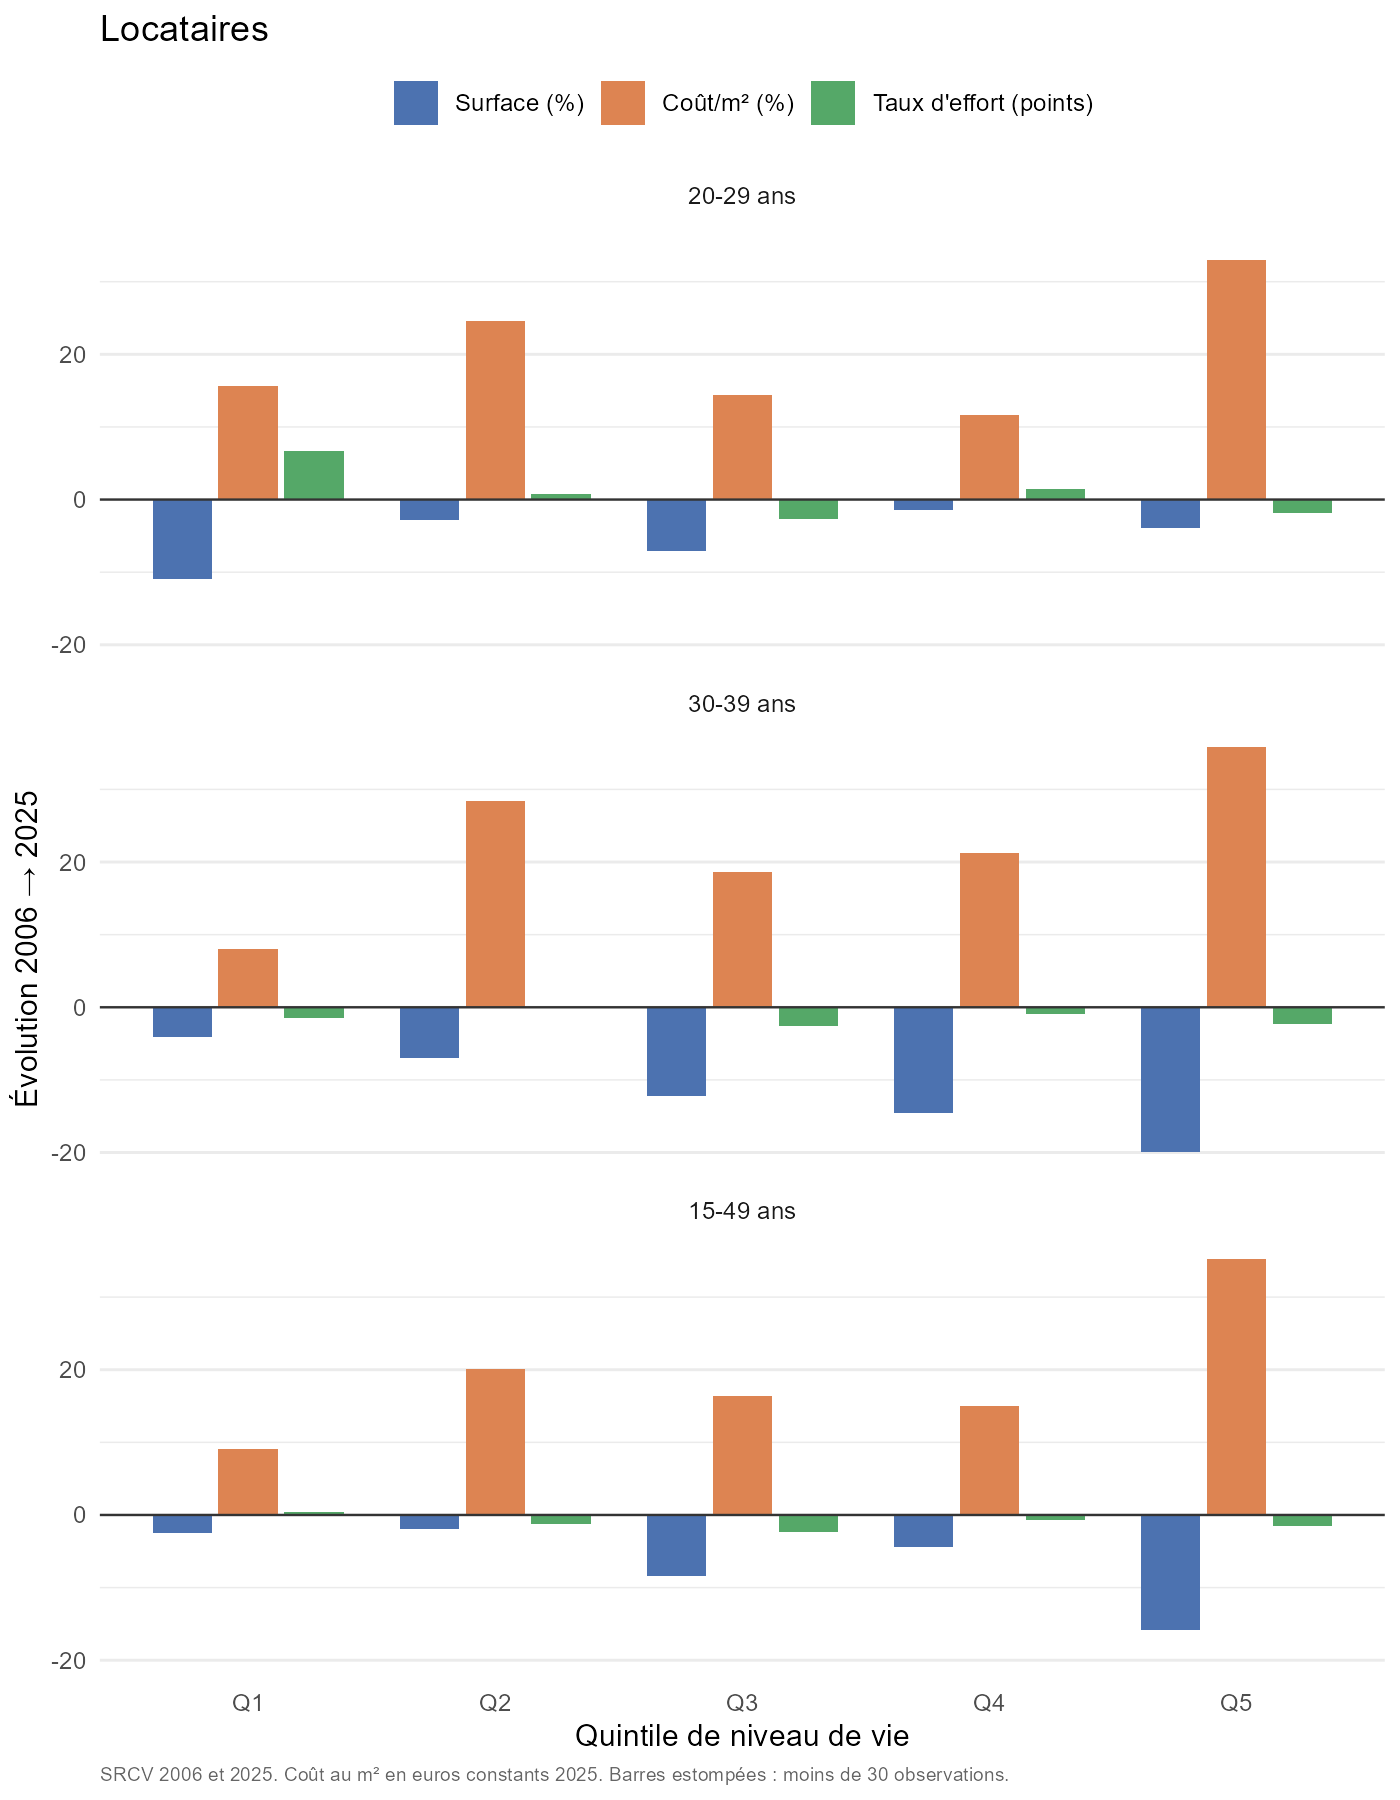
\includegraphics[width=\linewidth]{graph_quintiles_locataires}
		\caption{Prix et surface par quintile}\label{fig:loc_quintile}
	\end{minipage}
	\hfill
	\begin{minipage}{0.48\textwidth}
		\centering
		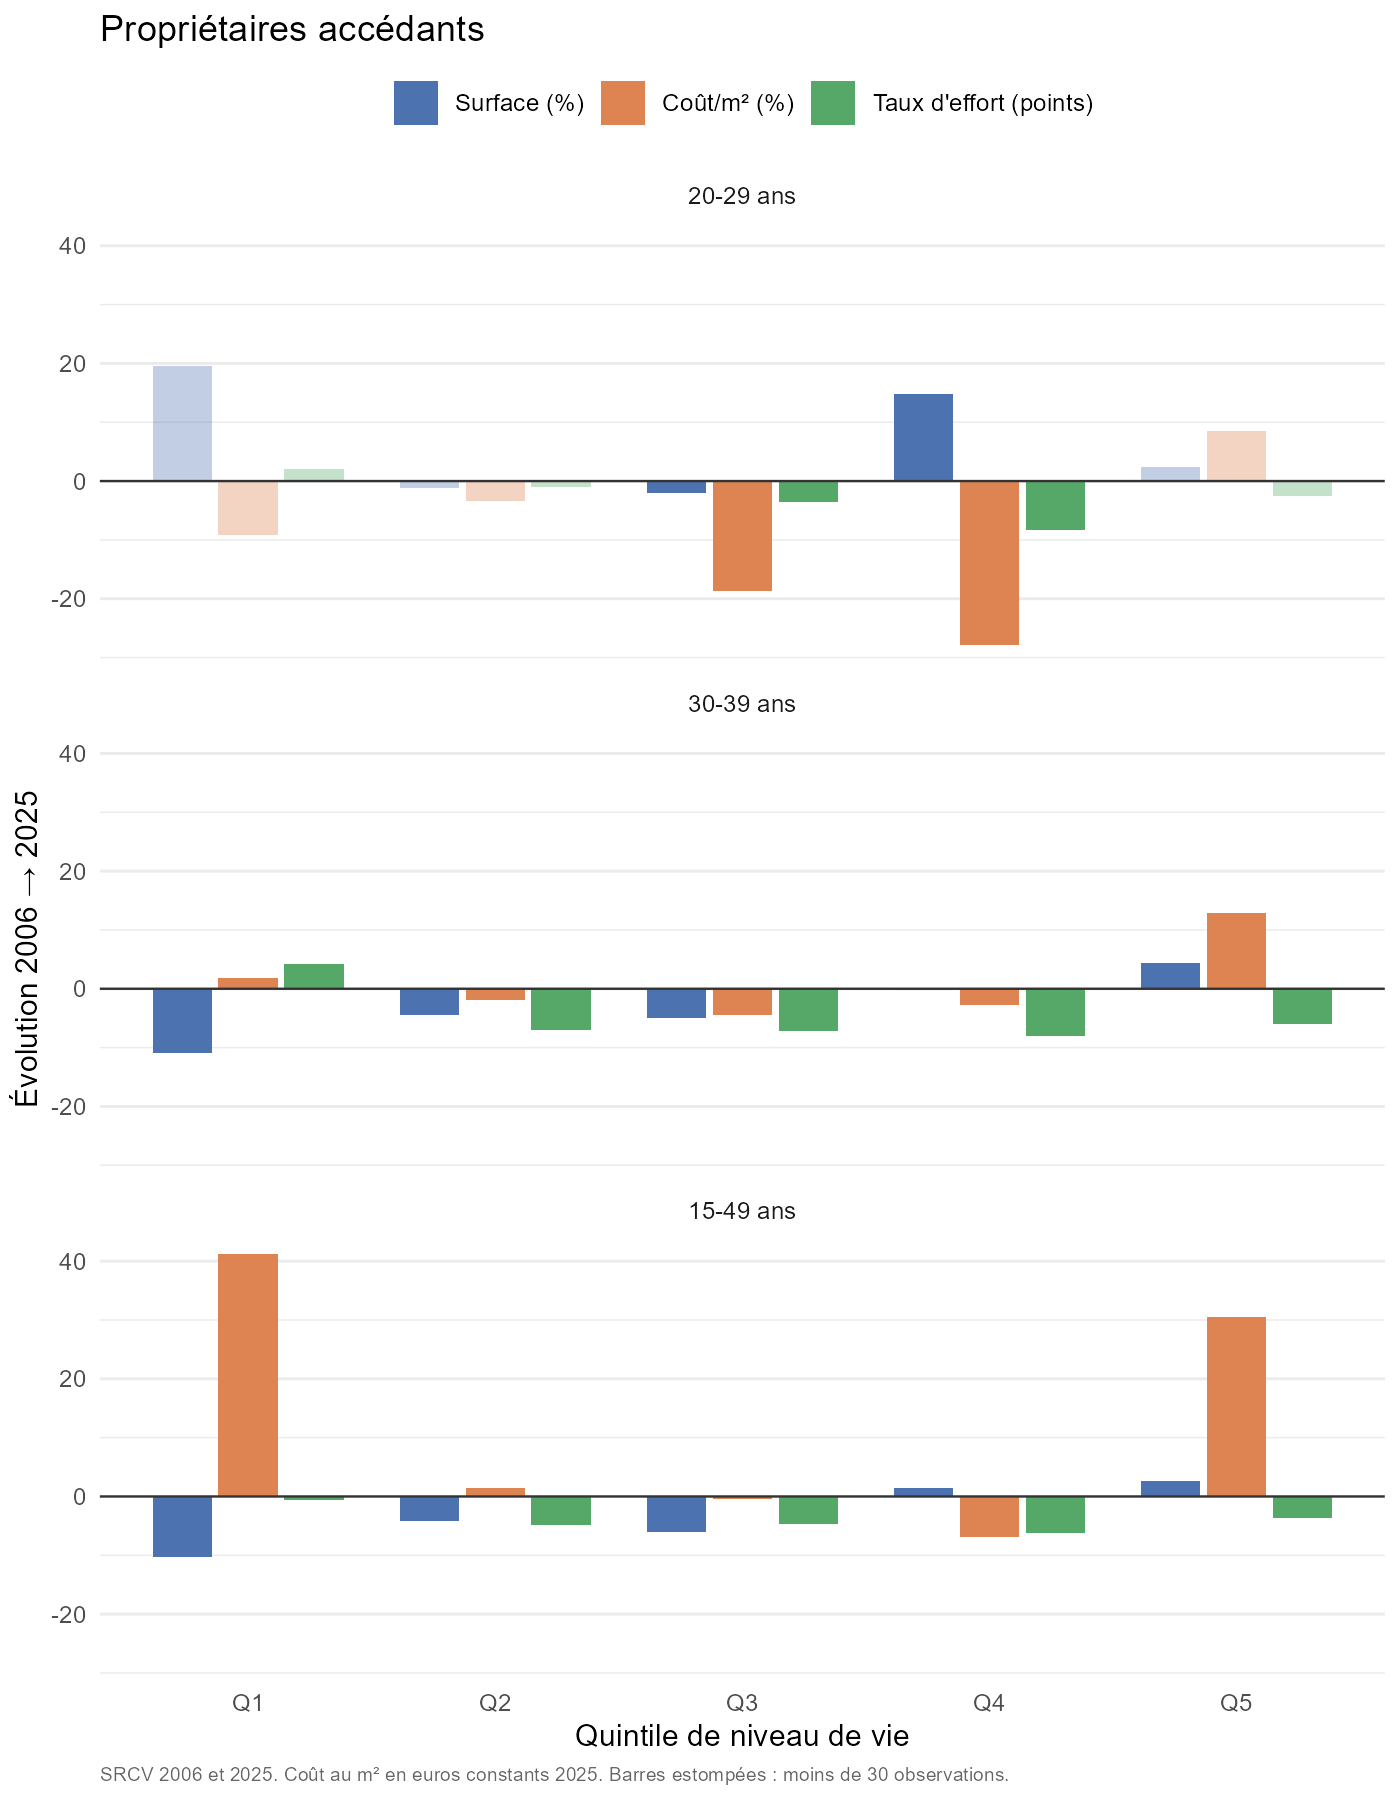
\includegraphics[width=\linewidth]{graph_quintiles_accedants}
		\caption{Prix et surface par quintile}\label{fig:acc_quintile}
	\end{minipage}
\end{figure} 

\bigskip

\noindent On remarque que globalement le taux d'effort est resté stable entre 2006 et 2025 pour les ménages français entre 20 et 39 ans, et globalement on retrouve les mêmes variations que lors des calculs par classe d'âge. Les locataires accusent une baisse de surface avec une hausse des prix, quand les propriétaires restent globalement stables sur tous les aspects, hormis quelques valeurs aberrantes. Les principaux enseignements sont que les quintiles les plus touchés sont les plus élevés chez les locataires de 30-39 ans et le quintile le moins élevé chez les 20-29 ans. Le dernier quintile des 30-39 ans a perdu 20\% de surface pour un prix au m$^2$ qui a bondi de plus de 30\% sur 20 ans. Le 2e quintile a moins subit sur la surface de son logement mais accuse une hausse de près de 30\% du prix au m$^2$ également. \\

\noindent Nous avons donc vu que l'évolution du marché immobilier a affecté de manière hétérogène les ménages français, par rapport à 2006 les ménages qui ont le plus été impactés sont les locataires du 30 à 39, et plus particulièrement ceux des quintiles 3 à 5. Ils ont perdu jusqu'à 20\% de la surface de leur logement pour un prix plus élevé, bien que le prix ait augmenté un peu moins rapidement que les revenus, ce qui fait que le taux d'effort s'est légèrement contracté. Il faut donc retenir qu'à niveau de dépense constante du logement dans le revenu, les jeunes ménages français ont surtout perdu de l'espace, ce qui va dans le sens de MeilleurAgents (2022) qui montrait qu'un couple avec des revenus médians avait perdu 18m$^2$ de capacité d'achat dans les métropoles hors Paris.   

\subsection{la distribution des naissances par rapport aux logements}

Avant de chercher à mesurer un effet, il faut regarder à quoi ressemble la donnée brute. Nous nous plaçons désormais sur le champ qui nous servira jusqu'à la fin de cette partie : les ménages en couple dont la femme, personne de référence ou conjointe, a entre 15 et 49 ans. C'est la population « à risque » d'avoir un enfant, et la restreindre ainsi n'est pas un détail de méthode : sur l'ensemble des ménages, les résultats sont écrasés par des effets de composition, les retraités et les personnes seules occupant des logements dont la taille n'a évidemment aucun rapport avec une décision de procréation. Sur les huit vagues cumulées, ce champ compte 26\,480 observations et 2\,118 naissances\footnote{Une observation est un couple observé dans une vague. Les vagues 2014-2018 et 2022-2025 étant des panels, un même ménage peut apparaître plusieurs fois : les erreurs-types sont regroupées au niveau du ménage.}. \\

\noindent Nous séparons dès maintenant deux décisions que la littérature confond trop souvent : celle d'avoir un \textit{premier} enfant, prise par un couple qui n'en a encore aucun, et celle d'en avoir un \textit{de plus}. Il n'y a aucune raison a priori pour que le logement pèse de la même façon sur les deux. Le premier enfant se décide dans un logement choisi pour un couple, souvent petit et souvent loué ; le deuxième ou le troisième se décide dans un logement déjà dimensionné pour une famille. Les deux sous-populations sont d'ailleurs de tailles très différentes : 5\,921 couples sans enfant, pour 827 premières naissances, contre 20\,559 couples déjà parents, pour 1\,291 naissances de rang deux ou plus. Le tableau \ref{tab:quartiles_surface} croise le taux de naissance avec le quartile de surface du logement, séparément pour chacune de ces deux décisions. \\

\bigskip

\begin{table}[htbp]
	\centering
	\footnotesize
	\setlength{\tabcolsep}{4pt}
	\begin{threeparttable}
		\caption{Taux de naissance selon le quartile de surface du logement et le rang de la naissance}
		\label{tab:quartiles_surface}
		\begin{tabular}{llrrrrr}
			\toprule
			& Quartile & \multicolumn{1}{c}{\shortstack{Surface\\médiane (m\textsuperscript{2})}}
			& \multicolumn{1}{c}{\shortstack{Taux de\\naissance (\%)}}
			& \multicolumn{1}{c}{\shortstack{Âge moyen\\de la femme}}
			& \multicolumn{1}{c}{\shortstack{Niveau de vie\\(k\texteuro/an/UC)}}
			& \multicolumn{1}{c}{\shortstack{Part de\\locataires (\%)}} \\
			\midrule
			\multirow{4}{*}{\textit{Premier enfant}}
			& Q1 & 45  & \textcolor{srcv3}{8,2}  & 28,3 & 28,7 & 79,0 \\
			& Q2 & 65  & 18,3 & 29,9 & 29,8 & 70,0 \\
			& Q3 & 84  & 17,7 & 31,5 & 33,0 & 47,1 \\
			& Q4 & 120 & 18,8 & 35,0 & 35,8 & 21,6 \\
			\addlinespace
			\multirow{4}{*}{\textit{Rang 2 et plus}}
			& Q1 & 70  & 11,0 & 36,3 & 24,4 & 61,8 \\
			& Q2 & 91  & 7,7  & 38,3 & 26,5 & 34,8 \\
			& Q3 & 120 & 6,5  & 39,3 & 30,3 & 14,1 \\
			& Q4 & 155 & 5,7  & 40,1 & 35,2 & 6,1 \\
			\bottomrule
		\end{tabular}
		\begin{tablenotes}[flushleft]\scriptsize
			\item \textit{Champ} : ménages en couple dont la femme (personne de référence ou
			conjointe) a 15 à 49 ans, France entière, vagues 2006, 2010, 2014, 2018, 2024 et 2025.
			\item \textit{Lecture} : les quartiles de surface sont calculés séparément dans chacune
			des deux sous-populations, la distribution des surfaces n'étant pas la même selon que
			le couple a déjà des enfants ou non. Parmi les couples sans enfant logés dans le
			quartile le plus petit (médiane 45 m\textsuperscript{2}), 8,2\,\% déclarent une naissance,
			contre 18,3\,\% dans le quartile suivant.
			\item \textit{Millésimes} : 2022 et 2023 sont écartées de tous les taux pondérés de
			cette étude (anomalie de pondération documentée en annexe \ref{annexe3}). Elles restent
			en revanche dans les modèles, où la distorsion est absorbée par les effets fixes d'année.
			\item \textit{Source} : Insee, SRCV 2006-2025, calculs de l'auteur.
		\end{tablenotes}
	\end{threeparttable}
\end{table}

\bigskip

\noindent Le contraste entre les deux moitiés du tableau est frappant. Chez les couples déjà parents, le taux de naissance \textit{décroît} régulièrement avec la surface, de 11,0\,\% dans le plus petit quartile à 5,7\,\% dans le plus grand : lu naïvement, il faudrait en conclure qu'habiter grand décourage d'avoir un enfant de plus. Ce n'est bien sûr qu'un artefact de composition, la colonne des âges le dit assez, les ménages du dernier quartile ont en moyenne quatre ans de plus que ceux du premier et sont largement sortis de la fenêtre où l'on agrandit sa famille. Chez les couples sans enfant, en revanche, la relation s'inverse et prend une forme qui n'est pas celle d'une pente : le quartile le plus petit décroche à 8,2\,\%, quand les trois autres se tiennent entre 17,7 et 18,8\,\% sans les départager. Autrement dit ce n'est pas « plus c'est grand, plus on fait d'enfants », c'est plutôt « en dessous d'un certain seuil, on n'en fait pas ». Ce seuil se situe quelque part entre 50 et 60 m$^2$, soit la surface d'un logement conçu pour deux personnes et pour deux personnes seulement ; nous le localiserons plus précisément au §\ref{sec:surface}. Là encore l'âge et le revenu vont dans le même sens et il faudra les contrôler avant de conclure quoi que ce soit, mais l'écart de dix points entre le premier et le deuxième quartile est trop grand pour être ignoré. \\

\noindent Le second fait qui ressort de ces données est l'écart entre locataires et propriétaires accédants, et surtout la manière dont il évolue. Le tableau \ref{tab:naiss_statut_rang} reprend le taux de naissance par statut d'occupation et par rang, vague par vague. \\

\bigskip

\begin{table}[htbp]
	\centering
	\footnotesize
	\setlength{\tabcolsep}{5pt}
	\begin{threeparttable}
		\caption{Taux de naissance par statut d'occupation et rang de la naissance, 2006-2025 (\%)}
		\label{tab:naiss_statut_rang}
		\begin{tabular}{lrrrrcrr}
			\toprule
			& \multicolumn{4}{c}{Module « événements »} & & \multicolumn{2}{c}{Fichier individus} \\
			\cmidrule(lr){2-5} \cmidrule(lr){7-8}
			& 2006 & 2010 & 2014 & 2018 & & 2024 & 2025 \\
			\midrule
			\multicolumn{8}{l}{\textit{Premier enfant}} \\
			Locataires              & 13,8 & 15,7 & 17,9 & 12,8 & & 12,7 & 8,4 \\
			Propriétaires accédants & 21,2 & 21,4 & 22,3 & 21,7 & & 16,0 & 18,4 \\
			\textit{Écart (points)} & \textit{+7,3} & \textit{+5,7} & \textit{+4,4} & \textit{+8,9} & & \textit{+3,3} & \textit{+10,0} \\
			\addlinespace
			\multicolumn{8}{l}{\textit{Rang 2 et plus}} \\
			Locataires              & 12,0 & 12,0 & 12,9 & 12,1 & & 10,4 & 7,0 \\
			Propriétaires accédants & 6,8 & 9,2 & 8,0 & 8,2 & & 4,6 & 5,0 \\
			\textit{Écart (points)} & \textit{-5,2} & \textit{-2,8} & \textit{-4,9} & \textit{-3,9} & & \textit{-5,8} & \textit{-2,0} \\
			\bottomrule
		\end{tabular}
		\begin{tablenotes}[flushleft]\scriptsize
			\item \textit{Champ} : ménages en couple dont la femme a 15 à 49 ans, France entière.
			Les propriétaires non accédants ne sont pas reportés (effectifs faibles et population
			nettement plus âgée) mais figurent en annexe \ref{annexe2}.
			\item \textit{Lecture} : en 2025, 8,4\,\% des couples locataires sans enfant déclarent
			une naissance, contre 18,4\,\% des couples accédants sans enfant, soit un écart de
			10,0 points.
			\item \textbf{Rupture de mesure} : la naissance est lue dans le module « événements »
			du fichier ménages jusqu'en 2018, et reconstruite depuis le fichier individus
			(présence d'un enfant né en N ou N-1) à partir de 2022, ce module ayant disparu des
			fichiers de production et de recherche. Les \textit{niveaux} ne sont donc pas
			comparables de part et d'autre de cette rupture ; les \textit{écarts entre statuts}
			au sein d'une même vague le sont, puisqu'ils sont mesurés avec la même définition.
			\item \textit{Source} : Insee, SRCV 2006-2025, calculs de l'auteur.
		\end{tablenotes}
	\end{threeparttable}
\end{table}

\bigskip

\noindent Ce tableau contient à lui seul l'essentiel de ce que nous allons chercher à établir. Pour le premier enfant, les couples accédants ont systématiquement une probabilité de naissance supérieure à celle des locataires, de 3 à 10 points selon les vagues, et l'écart est le plus large de toute la série en 2025. Pour les enfants de rang deux et plus, le signe s'inverse : ce sont les locataires qui ont le taux le plus élevé. Nous verrons que cette inversion n'est qu'un effet d'âge — les couples accédants déjà parents sont nettement plus avancés dans leur vie féconde — alors que l'avantage des accédants pour le premier enfant, lui, ne s'explique ni par l'âge ni par le revenu. \\

\noindent Il faut cependant se garder de lire l'évolution temporelle de ces taux. La chute apparente du taux de naissance des locataires sans enfant, de 17,9\,\% en 2014 à 8,4\,\% en 2025, mélange une baisse réelle et un changement de définition de la variable de naissance intervenu entre 2018 et 2022. Nous ne nous appuierons donc jamais, dans ce qui suit, sur la comparaison des \textit{niveaux} de natalité mesurés dans SRCV avant et après cette rupture. Pour tout ce qui touche à l'ampleur de la baisse de la natalité, nous utiliserons l'indicateur conjoncturel de fécondité publié par l'Insee, et nous réserverons les données SRCV à ce qu'elles mesurent de manière homogène sur vingt ans : les conditions de logement, et le lien entre ces conditions et la probabilité d'une naissance à un instant donné.

\newpage
	
\section{Le logement pèse-t-il sur la décision d'avoir un enfant ?}

Nous avons décrit jusqu'ici l'évolution des conditions de logement, et nous avons vu que les jeunes ménages locataires avaient surtout perdu de l'espace. Reste la question qui nous intéresse vraiment : est-ce que cela se traduit par des naissances en moins ? La réponse ne va pas de soi, et il faut résister à la tentation de conclure d'une corrélation. Les couples qui habitent grand sont aussi ceux qui sont plus âgés, plus aisés, plus souvent propriétaires, plus souvent installés dans une commune où l'on fait plus d'enfants qu'ailleurs. Chacune de ces caractéristiques suffirait à produire une corrélation entre surface et natalité sans qu'aucun mètre carré n'ait jamais fait naître personne. \\

\noindent Nous procédons donc en quatre temps. Nous mesurons d'abord l'effet de la \textit{quantité} de logement — la surface — en séparant la décision d'avoir un premier enfant de celle d'en avoir un de plus. Nous examinons ensuite si le statut d'occupation joue en propre, en le dépouillant l'un après l'autre de l'âge, du rang de naissance, du revenu et des conditions de logement. Nous regardons alors si l'effet est le même partout sur le territoire, ou s'il se concentre là où le marché est tendu. Nous terminons par la question qui donne son titre à cette étude : la fécondité française a reculé de près de 22\,\% entre 2010 et 2025, quelle part de ce recul le logement peut-il porter ?

\subsection{Ce que l'on peut mesurer, et ce que l'on ne peut pas}\label{sec:methode}

Le modèle que nous estimons est un probit pondéré sur la probabilité qu'un couple déclare une naissance, empilé sur les huit vagues avec des effets fixes d'année, et dont les erreurs-types sont regroupées au niveau du ménage puisque les vagues 2014-2018 et 2022-2025 réinterrogent les mêmes ménages. Tous les résultats sont présentés en effets marginaux moyens, exprimés en points de pourcentage de probabilité de naissance : un effet de $+0{,}5$ point sur un taux de base de 8,9\,\% représente une hausse relative d'environ 6\,\%. \\

\noindent Le point de méthode le plus important tient à la manière dont nous entrons le logement dans le modèle. Le taux d'effort, qui était l'angle initial de ce travail, est le produit de trois grandeurs : le prix au mètre carré, la surface consommée et l'inverse du revenu. L'agréger en un seul ratio revient à contraindre ces trois canaux à agir dans les mêmes proportions, ce qui n'a aucune raison d'être vrai\footnote{Nous avons estimé les modèles en taux d'effort dans une première version de ce travail : le coefficient est non significatif dans les huit vagues prises séparément comme dans la coupe empilée, et le reste quel que soit le statut d'occupation. Ce résultat nul n'est pas informatif pour autant, il agrège trois effets qui peuvent se compenser.}. Nous les séparons donc, en faisant entrer simultanément le prix au mètre carré, la surface et le niveau de vie du ménage. L'effet de la surface se lit alors « à prix au mètre carré et à revenu donnés », c'est-à-dire à qualité de marché comparable. Nous avons vérifié que la conclusion ne tient pas à cette convention : en tenant fixe le budget logement total plutôt que le prix unitaire — ce qui revient à comparer un grand logement bon marché à un petit logement cher, donc à déplacer le ménage vers la périphérie plutôt qu'à augmenter sa dépense — l'effet estimé est le même à un centième de point près. \\

\noindent Les contrôles de composition du ménage, eux, appellent une précaution qui n'est pas toujours prise. Le nombre d'enfants et la taille du ménage, tels qu'ils figurent dans les fichiers, \textit{comptent le nouveau-né} : contrôler par ces variables reviendrait à expliquer la naissance par sa propre conséquence. Nous reconstruisons donc systématiquement des versions antérieures à la naissance, et c'est également sur cette base que sont définis les couples « sans enfant » du premier rang. \\

\noindent Reste la difficulté de fond, celle que ni les contrôles ni la taille de l'échantillon ne règlent : \textbf{l'anticipation}. Un couple qui projette un enfant déménage souvent \textit{avant} qu'il n'arrive. La causalité court alors de la naissance vers le logement, et non l'inverse, et n'importe quel modèle en coupe attribuera au mètre carré ce qui revient au projet parental. Le phénomène est mesurable dans nos données : parmi les couples déjà parents, 28,6\,\% de ceux qui déclarent une naissance se sont installés dans leur logement depuis moins de trois ans, contre 14,5\,\% des autres, soit exactement le double. Chez les couples sans enfant l'écart est bien plus modeste — 45,2\,\% contre 42,0\,\% — ce qui est cohérent avec l'idée qu'on emménage pour former un couple avant d'emménager pour l'agrandir. Notre parade consiste à ré-estimer tous les modèles sur les seuls ménages installés depuis \textbf{au moins trois ans}, chez qui le logement est prédéterminé et ne peut plus être une conséquence de la naissance à venir. Nous avons vérifié sur le panel que le résultat ne dépend pas du seuil retenu, de deux à cinq ans.

\subsection{La surface compte, et surtout pour le premier enfant}\label{sec:surface}

Le tableau \ref{tab:effet_surface} donne les effets marginaux de la surface, du prix au mètre carré et du niveau de vie, pour l'ensemble du champ puis séparément selon le rang de la naissance, d'abord sur tous les couples puis sur les seuls ménages installés depuis au moins trois ans. \\

\bigskip

\begin{table}[htbp]
	\centering
	\footnotesize
	\setlength{\tabcolsep}{4pt}
	\begin{threeparttable}
		\caption{Effet du logement sur la probabilité de naissance, par rang (effets marginaux moyens, en points de pourcentage)}
		\label{tab:effet_surface}
		\begin{tabular}{lrrr}
			\toprule
			& \multicolumn{1}{c}{Ensemble} & \multicolumn{1}{c}{Premier enfant} & \multicolumn{1}{c}{Rang 2 et plus} \\
			\midrule
			\multicolumn{4}{l}{\textit{A. Tous les couples}} \\
			Surface (+10 m\textsuperscript{2})            & +0,53\sym{***} & +0,89\sym{***} & +0,40\sym{***} \\
			\quad \textit{intervalle de confiance à 95\,\%} & \textit{[0,40 ; 0,65]} & \textit{[0,54 ; 1,24]} & \textit{[0,29 ; 0,52]} \\
			Coût au m\textsuperscript{2} (+1 \texteuro/mois) & +0,00 & -0,02 & +0,01\sym{\dag} \\
			Niveau de vie (+10 k\texteuro/an/UC)         & -1,64\sym{**} & -2,25\sym{\dag} & -1,59\sym{**} \\
			\addlinespace
			Observations                                  & 26\,480 & 5\,921 & 20\,559 \\
			Naissances                                    & 2\,118 & 827 & 1\,291 \\
			Taux de naissance de référence (\%)           & 8,9 & 14,5 & 6,9 \\
			\addlinespace
			\midrule
			\multicolumn{4}{l}{\textit{B. Ménages installés depuis 3 ans ou plus (logement prédéterminé)}} \\
			Surface (+10 m\textsuperscript{2})            & +0,38\sym{***} & +0,73\sym{***} & +0,31\sym{***} \\
			\quad \textit{intervalle de confiance à 95\,\%} & \textit{[0,26 ; 0,50]} & \textit{[0,33 ; 1,13]} & \textit{[0,19 ; 0,42]} \\
			Coût au m\textsuperscript{2} (+1 \texteuro/mois) & +0,01 & -0,00 & +0,01\sym{\dag} \\
			Niveau de vie (+10 k\texteuro/an/UC)         & -1,47\sym{***} & -2,82\sym{***} & -1,21\sym{*} \\
			\addlinespace
			Observations                                  & 21\,191 & 3\,444 & 17\,747 \\
			Naissances                                    & 1\,413 & 472 & 941 \\
			Taux de naissance de référence (\%)           & 7,4 & 13,8 & 5,8 \\
			\addlinespace
			\midrule
			\multicolumn{4}{l}{\textit{C. Pour mémoire : ménages installés depuis moins de 3 ans}} \\
			Surface (+10 m\textsuperscript{2})            & +0,93\sym{***} & --- & --- \\
			Observations / naissances                     & 5\,284 / 705 & --- & --- \\
			\bottomrule
		\end{tabular}
		\begin{tablenotes}[flushleft]\scriptsize
			\item \sym{***} $p<0{,}001$ ; \sym{**} $p<0{,}01$ ; \sym{*} $p<0{,}05$ ; \sym{\dag} $p<0{,}10$.
			\item \textit{Champ} : ménages en couple dont la femme a 15 à 49 ans, France entière,
			huit vagues empilées (2006 à 2025).
			\item \textit{Modèle} : probit pondéré, effets fixes d'année, erreurs-types regroupées
			au niveau du ménage. Contrôles : statut d'occupation, âge de la femme et son carré,
			déménagement dans l'année, catégorie socioprofessionnelle, degré d'urbanisation, ZEAT ;
			plus, hors modèle du premier enfant, le nombre d'enfants et la taille du ménage
			\textit{avant} la naissance.
			\item \textit{Lecture} : chez les couples sans enfant installés depuis au moins trois
			ans, dix mètres carrés supplémentaires sont associés à une probabilité de première
			naissance supérieure de 0,73 point, sur un taux de référence de 13,8\,\%, soit une
			hausse relative de 5,3\,\%.
			\item \textit{Source} : Insee, SRCV 2006-2025, calculs de l'auteur.
		\end{tablenotes}
	\end{threeparttable}
\end{table}

\bigskip

\noindent Trois enseignements se dégagent. Le premier est que \textbf{c'est bien la quantité de logement qui joue, et non son prix}. L'effet du coût au mètre carré est nul, quel que soit le sous-champ retenu, et son intervalle de confiance est suffisamment serré pour qu'on puisse écarter un effet de taille appréciable. C'est en soi un résultat qui mérite d'être souligné, car le débat public sur logement et natalité est presque entièrement formulé en termes de prix. Nos données disent que ce n'est pas le prix qui compte mais ce que le prix permet d'acheter, ce qui n'est pas la même chose et n'appelle pas les mêmes réponses de politique publique. \\

\noindent Le deuxième enseignement est que \textbf{l'effet de la surface est plus de deux fois plus fort pour le premier enfant que pour les suivants} : $+0{,}89$ point contre $+0{,}40$ point pour dix mètres carrés. Rapporté aux taux de base respectifs, l'écart est un peu atténué mais reste substantiel. Estimé dans un modèle unique avec une interaction, ce qui permet de tester formellement la différence plutôt que de comparer deux échantillons, le contraste est plus marqué encore — $+1{,}17$ point contre $+0{,}34$ point — et la différence est significative au seuil de 1\,\% ($p = 0{,}005$). Ce résultat est cohérent avec ce que montrait le tableau \ref{tab:quartiles_surface} : la contrainte de logement se joue à l'entrée dans la parentalité, dans un logement dimensionné pour deux, et beaucoup moins ensuite. \\

\noindent Ce deuxième enseignement demande toutefois une précision, car la relation n'a pas la forme d'une pente. En remplaçant la surface continue par cinq tranches, on voit qu'il s'agit d'une \textbf{marche} plutôt que d'une pente. Les bornes 50, 70, 90 et 120 m$^2$ du tableau \ref{tab:seuil} sont des nombres ronds posés a priori ; nous vérifions ensuite où la marche se situe réellement. Le tableau donne les écarts par rapport à la tranche de référence, celle des logements de 70 à 89 m$^2$. \\

\bigskip

\begin{table}[htbp]
	\centering
	\footnotesize
	\setlength{\tabcolsep}{4pt}
	\begin{threeparttable}
		\caption{Écart de probabilité de naissance par tranche de surface, et évolution de l'exposition (points de pourcentage)}
		\label{tab:seuil}
		\begin{tabular}{lrrrr}
			\toprule
			\multicolumn{5}{l}{\textit{A. Écart par rapport aux logements de 70 à 89 m\textsuperscript{2}}} \\
			Tranche de surface & \multicolumn{1}{c}{Ensemble}
			& \multicolumn{1}{c}{\shortstack{Premier\\enfant}}
			& \multicolumn{1}{c}{\shortstack{Premier enfant,\\installés 3 ans +}}
			& \multicolumn{1}{c}{\shortstack{Rang 2\\et plus}} \\
			\midrule
			Moins de 50 m\textsuperscript{2}  & -5,98\sym{***} & -9,07\sym{***} & -7,76\sym{***} & -2,57\sym{*} \\
			50 à 69 m\textsuperscript{2}      & -1,95\sym{**}  & -1,33          & -2,38          & -1,55\sym{*} \\
			70 à 89 m\textsuperscript{2}      & \textit{réf.}  & \textit{réf.}  & \textit{réf.}  & \textit{réf.} \\
			90 à 119 m\textsuperscript{2}     & +1,12\sym{\dag}& +3,53\sym{\dag}& +4,70\sym{\dag}& +0,58 \\
			120 m\textsuperscript{2} et plus  & +2,28\sym{**}  & +4,07\sym{\dag}& +1,77          & +2,04\sym{**} \\
			\addlinespace
			Taux de naissance de référence (\%) & 8,9 & 14,5 & 13,8 & 6,9 \\
			\addlinespace
			\midrule
			\multicolumn{5}{l}{\textit{B. Répartition des couples sans enfant par tranche (\%)}} \\
			& \multicolumn{1}{c}{2010} & \multicolumn{1}{c}{2025} & \multicolumn{1}{c}{Écart} & \\
			\midrule
			Moins de 50 m\textsuperscript{2}  & 15,1 & 19,1 & \textbf{+4,0} & \\
			50 à 69 m\textsuperscript{2}      & 28,8 & 25,7 & -3,1 & \\
			70 à 89 m\textsuperscript{2}      & 24,7 & 21,9 & -2,8 & \\
			90 à 119 m\textsuperscript{2}     & 20,2 & 19,7 & -0,5 & \\
			120 m\textsuperscript{2} et plus  & 11,3 & 13,5 & +2,2 & \\
			\bottomrule
		\end{tabular}
		\begin{tablenotes}[flushleft]\scriptsize
			\item \sym{***} $p<0{,}001$ ; \sym{**} $p<0{,}01$ ; \sym{*} $p<0{,}05$ ; \sym{\dag} $p<0{,}10$.
			\item \textit{Champ} : ménages en couple dont la femme a 15 à 49 ans. Panneau A : huit
			vagues empilées. Panneau B : 2010 et 2025, couples sans enfant uniquement.
			\item \textit{Lecture} : un couple sans enfant logé dans moins de 50 m\textsuperscript{2}
			a une probabilité de première naissance inférieure de 9,07 points à celle d'un couple
			logé entre 70 et 89 m\textsuperscript{2}, toutes choses égales par ailleurs, sur un taux
			de référence de 14,5\,\%.
			\item \textit{Modèle} : mêmes contrôles que le tableau \ref{tab:effet_surface}, la surface
			continue étant remplacée par les cinq tranches.
			\item \textit{Bornes} : posées a priori. En tranches fines, le décrochage est graduel sous
			60 m\textsuperscript{2} et nul au-dessus, et la recherche de point de rupture retient
			60 m\textsuperscript{2} (texte, script R/30).
			\item \textit{Source} : Insee, SRCV 2006-2025, calculs de l'auteur.
		\end{tablenotes}
	\end{threeparttable}
\end{table}

\bigskip

\noindent Chez les couples sans enfant, être logé sous 50 mètres carrés est associé à une probabilité de première naissance inférieure de 9,1 points à celle des couples logés entre 70 et 89 mètres carrés, soit près des deux tiers du taux de référence. Le résultat tient chez les seuls ménages installés depuis trois ans ou plus, où l'écart reste de 7,8 points. Au-dessus de ce seuil, en revanche, la surface ne départage plus grand-chose : passer de la tranche 50-69 à la tranche de référence ne produit aucun écart significatif, et les deux tranches supérieures ne se distinguent qu'à la marge. Chez les couples déjà parents, la même marche existe mais elle est trois fois et demie plus faible, à $-2{,}6$ points. Ce que le logement contraint n'est donc pas la taille de la famille, c'est le fait d'en fonder une dans un logement conçu pour deux. \\

\noindent Reste à savoir si cette marche est un fait ou un choix de bornes. Trois vérifications répondent\footnote{Script \texttt{R/30}. Les trois portent sur les couples sans enfant, tous puis installés depuis trois ans ou plus, avec les contrôles du tableau \ref{tab:effet_surface}.}. En tranches fines de dix mètres carrés, l'écart avec la référence est de $-11$ points sous 40 m$^2$, $-8$ entre 40 et 49, $-6$ entre 50 et 59, puis nul à partir de 60 m$^2$ ($+2{,}3$ point entre 60 et 69, non significatif) : la probabilité de première naissance décroît graduellement sous 60 m$^2$ et ne bouge plus au-dessus. En déplaçant la borne basse de 40 à 60 m$^2$, l'écart de la tranche la plus petite reste compris entre $-8$ et $-11$ points quelle que soit la borne, et la tranche intermédiaire ne se distingue plus de la référence dès que la borne atteint 55 m$^2$. Enfin, une recherche de point de rupture — une indicatrice « moins de $c$ mètres carrés » pour $c$ de 35 à 75 — retient $c = 60$ m$^2$, borne de déviance minimale dans les quatre variantes, avec un écart de $-8$ à $-10$ points qui subsiste même lorsque la pente linéaire est conservée dans le modèle. \textbf{La marche est donc estimée et non posée, et elle se situe à 60 m$^2$ plutôt qu'à 50} ; les tranches du tableau \ref{tab:seuil} la coupent un peu bas, ce qui rend le résultat conservateur. La part des couples sans enfant logés sous 60 m$^2$ est passée de 27,6 à 30,6\,\% entre 2010 et 2025, contre 15,1 à 19,1\,\% sous 50 m$^2$ ; nous mesurerons au §\ref{sec:decompo} ce que la décomposition doit à la borne retenue. \\

\noindent Cette forme a une conséquence directe pour la suite de l'étude, et le panneau B du tableau la donne : une surface \textit{moyenne} peut rester parfaitement stable pendant que la part des ménages situés \textit{sous} le seuil augmente. C'est exactement ce qui s'est produit. La part des couples sans enfant logés dans moins de 50 m$^2$ est passée de 15,1\,\% en 2010 à 19,1\,\% en 2025, quatre points de plus, pendant que les tranches intermédiaires se vidaient et que le haut de la distribution s'étoffait légèrement. La distribution s'est polarisée sans que sa moyenne bouge. Nous verrons au §\ref{sec:decompo} que ce point de spécification change d'un facteur dix l'ampleur du canal « surface » dans la décomposition finale. \\

\noindent Le troisième enseignement est plus inattendu et nous y reviendrons : le niveau de vie a un effet \textbf{négatif} et significatif sur la probabilité de naissance, de l'ordre de $-1{,}5$ à $-2{,}8$ points pour dix mille euros de niveau de vie annuel supplémentaire. À logement, âge et catégorie sociale donnés, les couples les plus aisés font moins d'enfants, ce qui rejoint le constat descriptif que nous avions fait sur les taux de naissance par tranche de revenu. Nous ne l'interprétons pas comme un effet du revenu lui-même, mais plutôt comme la trace du coût d'opportunité : à revenu élevé correspondent des carrières où l'interruption coûte cher, et c'est l'un des points que nous reprendrons dans la partie consacrée à la politique familiale. \\

\noindent Il faut maintenant dire clairement ce que ces coefficients ne prouvent pas. Restreindre l'échantillon aux ménages installés depuis trois ans réduit l'effet de la surface d'environ 30\,\%, ce qui donne la mesure de la part imputable à l'anticipation : chez les seuls déménageurs récents, l'effet monte à $+0{,}93$ point, deux fois et demie celui des installés. Mais il ne l'annule pas, et l'effet reste très significatif. Nous disposons cependant d'un second dispositif, plus exigeant : le panel, qui suit les mêmes ménages d'une vague à l'autre et permet d'observer le logement en $t$ puis la naissance entre $t$ et $t+1$, dans le bon ordre temporel. Sur ce panel, restreint lui aussi aux ménages installés depuis au moins trois ans, l'effet de la surface est \textbf{nul} : $-0{,}007$ point pour dix mètres carrés, avec un intervalle de confiance qui exclut confortablement l'ordre de grandeur trouvé en coupe\footnote{L'effet minimum détectable de ce panel, à 5\,\% de risque et 80\,\% de puissance, est de 0,083 point pour dix mètres carrés, soit 1,5\,\% du taux de naissance. Le résultat nul n'est donc pas un manque de puissance : un effet de l'ampleur de celui estimé en coupe aurait été détecté.}. \\

\noindent Les deux dispositifs ne disent pas la même chose, et il serait malhonnête de choisir celui qui arrange. Le panel identifie mieux, puisque le logement y précède strictement la naissance ; mais il repose sur un dixième des naissances, sur les seules vagues chaînées, et sur une spécification qui n'est pas tout à fait celle de la coupe. Nous avons donc fait le test qui départage : estimer, sur l'échantillon même du panel — les couples observés en $t$ et en $t+1$ — exactement la spécification de la coupe, probit, prix au mètre carré, mêmes contrôles, en ne changeant que la naissance expliquée. Chez les ménages installés depuis trois ans ou plus, la surface en $t$ est associée à la naissance déclarée en $t$ ($+0{,}33$ point pour dix mètres carrés, $p < 0{,}001$, 5\,967 observations), mais pas à la naissance survenue entre $t$ et $t+1$ ($+0{,}06$ point, $p = 0{,}56$, sur les mêmes observations) ; chez les couples sans enfant installés, le signe s'inverse même ($-0{,}37$ point, non significatif)\footnote{Sur l'ensemble des couples du panel, sans restriction d'ancienneté, l'effet prospectif subsiste mais réduit de moitié ($+0{,}22$ contre $+0{,}40$ point), ce qui est cohérent avec la part d'anticipation par déménagement mesurée plus haut. La spécification initiale du panel (coût total, diplôme, actifs occupés, logit) donne la même chose sur les mêmes observations : $+0{,}09$ à $+0{,}11$ point chez les installés, non significatif. Script \texttt{R/29}.}. L'écart entre coupe et panel ne vient donc ni de la spécification, ni de l'échantillon chaîné, ni de la paramétrisation : il vient de l'ordre temporel. La surface est associée à une naissance récente ; elle ne prédit pas la naissance suivante. Cela se comprend mal comme une contrainte de logement, qui devrait jouer vers l'avant, et mieux comme la trace d'un logement choisi en fonction d'un projet de famille déjà formé, y compris chez des ménages qui n'ont pas déménagé depuis trois ans — l'anticipation peut précéder la naissance de plus de trois ans. Nous retenons donc la formulation prudente, et désormais mieux étayée : \textbf{l'association entre surface et première naissance est solide, robuste et bien caractérisée ; son interprétation causale, elle, ne l'est pas, et le panel plaide contre}. Nous verrons au §\ref{sec:decompo} que la question centrale de cette étude peut heureusement être tranchée sans avoir à départager les deux. \\

\noindent Une dernière vérification s'imposait, celle de la rupture de mesure de la naissance dont nous avons parlé plus haut. Si l'effet de la surface tenait à la façon dont la naissance est enregistrée, il ne devrait pas survivre des deux côtés de 2018. Il y survit. Estimé sur les seules vagues 2006 à 2018, où la naissance est lue dans le module « événements », il vaut $+0{,}65$ point pour dix mètres carrés ; estimé sur les seules vagues 2022 à 2025, où elle est reconstruite depuis le fichier individus, il vaut $+0{,}38$ point. L'écart entre les deux disparaît d'ailleurs presque entièrement dès qu'on les rapporte au taux de naissance de chaque période, plus élevé dans les vagues anciennes : dix mètres carrés valent alors 6,1\,\% du taux de naissance dans le premier cas et 5,8\,\% dans le second. Le résultat n'est donc ni un artefact de définition, ni le produit d'une seule période. \\

\noindent Deux dernières vérifications, de nature différente, visent à écarter que cet effet ne soit qu'un artefact d'autre chose. La première teste s'il s'agit bien de mètres carrés, et non simplement du fait d'habiter une maison plutôt qu'un appartement — les maisons étant en moyenne plus grandes. En ajoutant le type de logement en contrôle\footnote{Construit à partir de \texttt{HH010} (2006-2014) puis \texttt{TYPLOG} (2018-2025), deux variables dont la nomenclature change de sens sous le même nom entre 2018 et 2022 — le code « 5 » signifie « appartement en immeuble de 10 logements ou plus » dans la première version, « foyer pour personnes âgées ou étudiants » dans la seconde. Vérifié par un croisement des deux variables sur 2014, la seule vague où elles coexistent : bijection exacte sur les 11 384 ménages, aucune discordance une fois le bon code appliqué à chaque période. Champ renseigné pour 99,4\,\% des ménages. L'effet de la surface pour le premier enfant, ménages installés depuis trois ans ou plus, recule de 0,73 à 0,63 point pour dix mètres carrés ($-14$\,\%, $p = 0{,}003$ contre $p = 0{,}0004$ sans ce contrôle), la référence étant exactement la spécification du tableau \ref{tab:effet_surface} ; le type de logement lui-même, à surface égale, n'a pas d'effet propre détectable ($-2{,}3$ points, $p = 0{,}14$). Le résultat le plus robuste de cette section, le seuil à 50 m\textsuperscript{2} du tableau \ref{tab:seuil}, est presque insensible à ce contrôle ($-9{,}06$ contre $-8{,}83$ points), et l'avantage des accédants au premier enfant (tableau \ref{tab:escalier}, M5) passe de 5,4 à 5,0 points.} l'effet recule modestement mais reste très significatif. Il faut toutefois se garder de lire ce recul comme un artefact écarté : maison ou appartement fait partie du même choix de logement que la surface, et si l'effet de la surface passe en partie par « une maison avec un jardin », contrôler le type de logement retire une part légitime de l'effet et non un facteur de confusion. Les deux lectures sont possibles et nous ne les départageons pas ; l'ordre de grandeur du résultat, lui, n'en dépend pas. La seconde vérification s'attaque à un risque différent : que la surface déclarée par le ménage ne soit, en réalité, qu'un marqueur de la tension du marché local — auquel cas ce serait moins un effet du logement du ménage qu'un effet de contexte mal identifié. Nous construisons donc, à partir des transactions immobilières réelles DVF\,+ (Cerema, 2014-2025), un indice de prix au m\textsuperscript{2} par ZEAT et par année, totalement indépendant du logement occupé par chaque ménage\footnote{1,18 million de transactions exploitables (vente d'un seul bien, maison ou appartement, sur les 97 départements — la Moselle, le Bas-Rhin et le Haut-Rhin en sont absents, leur régime foncier particulier n'étant pas couvert par DVF\,+). Prix médian par ZEAT, année et type de bien, apparié au type du logement occupé par le ménage (maison ou appartement) : un indice mélangeant les deux serait dominé par la part d'appartements de chaque zone. Champ apparié à 93,8\,\% des ménages 2014-2025 (DVF\,+ ne couvre pas 2006-2010).} : l'effet de la surface est le même, qu'on l'ajoute ou non (0,59 contre 0,54 point pour le premier enfant sur ce sous-champ, un écart inférieur au tiers de l'erreur-type ; 0,38 contre 0,37 sur l'ensemble). C'est la seule conclusion que ce test autorise, et il faut dire pourquoi. L'indice ne varie qu'au niveau de la ZEAT, de l'année et du type de bien, et le modèle contient déjà des effets fixes de ZEAT et d'année : son coefficient propre n'est identifié que sur la déformation différentielle de 96 cellules, et son erreur-type varie du simple au double selon que l'on regroupe les observations au niveau du ménage ou de la cellule. Nous ne tirons donc rien de ce coefficient. Ce qui reste, et qui suffit ici, c'est que la surface individuelle ne recouvre pas un signal de marché mal identifié. \\

\noindent Il reste deux fragilités propres aux vagues 2022 à 2025, que nous avions signalées sans les traiter. La première est un \textbf{double comptage}. Dans ces fichiers, la naissance est reconstruite comme la présence d'un enfant né dans l'année ou l'année précédente ; un enfant né en 2022 est donc compté dans la vague 2022 et de nouveau dans la vague 2023 pour les ménages réinterrogés, et la moitié des naissances des vagues 2023 à 2025 sont dans ce cas. Les effets fixes d'année absorbent le niveau, pas la composition de ce qui est compté deux fois. La seconde est l'\textbf{anomalie de pondération} des vagues 2022 et 2023, documentée en annexe \ref{annexe3}, qui touche précisément les ménages avec nouveau-né et que les modèles conservaient au motif que les effets fixes l'absorbaient. Nous avons ré-estimé les résultats de cette partie sous cinq variantes\footnote{Script \texttt{R/28}. Variantes : naissance limitée aux enfants nés dans l'année d'enquête (cohorte incomplète) ; limitée aux enfants nés l'année précédente (cohorte complète, fenêtre de douze mois, la plus proche du module « événements ») ; dédupliquée, l'enfant né l'année précédente n'étant compté que si le ménage n'était pas déjà dans l'échantillon (chaque naissance compte une fois) ; référence sans les vagues 2022 et 2023 ; dédupliquée sans 2022 et 2023. Le rang et les contrôles pré-naissance sont recalculés dans chaque variante.}. L'effet de la surface pour le premier enfant, ménages installés, va de 0,64 à 0,81 point selon la variante, contre 0,73 en référence, et reste significatif dans toutes ; l'écart des couples logés sous 50 m$^2$ va de $-4{,}6$ à $-8{,}3$ points chez les installés, contre $-7{,}8$, significatif partout. L'avantage des accédants au premier enfant est plus sensible : il tombe à 2,4 points ($p = 0{,}05$) lorsque la naissance est limitée aux enfants nés dans l'année, mais se maintient entre 4,3 et 5,4 points dans les quatre autres variantes, dédupliquée comprise. La décomposition du §\ref{sec:decompo} est reprise sous chaque variante, et nous y reviendrons : aucune ne change la réponse.

\subsection{Locataire ou propriétaire : ni un effet d'âge, ni un effet de revenu}\label{sec:statut}

Le tableau \ref{tab:naiss_statut_rang} montrait un écart brut important entre accédants et locataires, positif pour le premier enfant et négatif pour les suivants. Pour savoir ce qu'il y a derrière, nous partons de l'écart brut et nous ajoutons les contrôles un par un, en lisant l'écart après chaque ajout. Si l'écart s'effondre lorsqu'on introduit l'âge, c'est un effet de cycle de vie ; s'il s'effondre lorsqu'on introduit le revenu, l'« effet propriétaire » n'était qu'un effet revenu déguisé ; s'il s'effondre lorsqu'on introduit la surface, c'est que le statut n'agissait que par le logement qu'il permet d'occuper. Le tableau \ref{tab:escalier} présente cet escalier. \\

\bigskip

\begin{table}[htbp]
	\centering
	\footnotesize
	\setlength{\tabcolsep}{4pt}
	\begin{threeparttable}
		\caption{Écart de probabilité de naissance des propriétaires accédants par rapport aux locataires, selon les contrôles introduits (points de pourcentage)}
		\label{tab:escalier}
		\begin{tabular}{lrrr}
			\toprule
			Contrôles introduits & \multicolumn{1}{c}{Ensemble} & \multicolumn{1}{c}{Premier enfant} & \multicolumn{1}{c}{Rang 2 et plus} \\
			\midrule
			M0 : statut seul (+ année)            & -2,36\sym{***} & +6,15\sym{***} & -3,63\sym{***} \\
			M1 : + âge de la femme                & -0,07          & +5,46\sym{***} & -1,49\sym{**} \\
			M2 : + rang et taille du ménage       & +0,06          & +5,44\sym{***} & -1,65\sym{***} \\
			M3 : + niveau de vie                  & +1,10\sym{*}   & +7,10\sym{***} & -0,75 \\
			M4 : + catégorie sociale et géographie & +1,65\sym{**}  & +6,87\sym{***} & -0,06 \\
			M5 : + surface et prix au m\textsuperscript{2} & +0,51 & +5,12\sym{***} & -1,05\sym{\dag} \\
			\addlinespace
			\midrule
			\multicolumn{4}{l}{\textit{Pour mémoire : propriétaires non accédants vs locataires}} \\
			M0 : statut seul (+ année)            & -6,45\sym{***} & -3,43\sym{*} & -6,72\sym{***} \\
			M1 : + âge de la femme                & -0,62          & +0,80        & -1,58\sym{\dag} \\
			M5 : jeu complet de contrôles         & -0,84          & +0,38        & -1,57\sym{\dag} \\
			\bottomrule
		\end{tabular}
		\begin{tablenotes}[flushleft]\scriptsize
			\item \sym{***} $p<0{,}001$ ; \sym{**} $p<0{,}01$ ; \sym{*} $p<0{,}05$ ; \sym{\dag} $p<0{,}10$.
			\item \textit{Champ} : ménages en couple dont la femme a 15 à 49 ans, France entière,
			huit vagues empilées ; 26\,480 observations et 2\,118 naissances pour l'ensemble.
			\item \textit{Lecture} : sans autre contrôle que l'année, les couples accédants sans
			enfant ont une probabilité de première naissance supérieure de 6,15 points à celle des
			couples locataires sans enfant. Une fois l'âge de la femme contrôlé, l'écart reste de
			5,46 points ; une fois le niveau de vie ajouté, il monte à 7,10 points.
			\item \textit{Modèle} : probit pondéré, effets fixes d'année, erreurs-types regroupées
			au niveau du ménage. Chaque ligne ajoute les contrôles aux précédents.
			\item \textit{Source} : Insee, SRCV 2006-2025, calculs de l'auteur.
		\end{tablenotes}
	\end{threeparttable}
\end{table}

\bigskip

\noindent La lecture de la première colonne est sans ambiguïté : \textbf{sur l'ensemble du champ, l'écart brut entre accédants et locataires est intégralement un effet d'âge}. Il vaut $-2{,}4$ points sans contrôle et devient nul, exactement nul, dès qu'on introduit l'âge de la femme. Le constat vaut de manière encore plus spectaculaire pour les propriétaires non accédants, dont le déficit apparent de $-6{,}4$ points s'évanouit lui aussi entièrement avec l'âge — ce qui n'a rien de surprenant s'agissant de ménages ayant fini de rembourser leur emprunt. Quiconque compare des taux de natalité par statut d'occupation sans contrôler l'âge ne mesure rien d'autre que la position des ménages dans leur cycle de vie. \\

\noindent Mais cette réponse globale masque deux réponses opposées. Chez les couples déjà parents, il n'y a effectivement rien : l'écart passe de $-3{,}6$ points à $-1{,}5$ avec l'âge, puis devient non significatif dès qu'on ajoute le revenu, et le reste ensuite. Chez les couples sans enfant, en revanche, \textbf{l'avantage des accédants est considérable et il résiste à tout}. Il vaut $+6{,}2$ points sans contrôle, soit une probabilité de première naissance supérieure de 42\,\% en relatif, et l'introduction de l'âge ne lui retire qu'un dixième de sa valeur, alors même que les femmes accédantes sans enfant ont en moyenne trois à quatre ans de plus que les locataires sans enfant. \\

\noindent Le passage de M2 à M3 est le plus instructif, et il répond directement à la question que nous nous posions : \textbf{non, l'effet propriétaire n'est pas un effet revenu sous-jacent}. Contrôler le niveau de vie ne réduit pas l'écart, il l'\textit{augmente}, de 5,4 à 7,1 points. La mécanique est celle que nous avons vue plus haut : le niveau de vie a un effet propre négatif sur la natalité, et les accédants sont nettement plus aisés que les locataires. Tant que le revenu n'est pas contrôlé, il tire donc l'écart vers le bas et masque une partie de l'avantage des accédants ; une fois neutralisé, l'avantage apparaît en entier. À revenu égal, être accédant plutôt que locataire est associé à une probabilité de première naissance supérieure de sept points, sur un taux de base de 14,5\,\%.\footnote{Un canal proche du revenu, mais distinct : le patrimoine financier. Un ménage peut avoir un flux de revenu modeste mais une épargne de précaution substantielle, ou l'inverse. SRCV interroge, sur les huit vagues, la détention de six produits financiers en tranches (livrets, assurance-vie, épargne logement, valeurs mobilières, PEA et autres placements) ; nous en tirons un score ordinal comparable entre vagues et l'ajoutons en contrôle, sur le sous-échantillon apparié (92,3\,\% du champ). Le résultat est le même que pour le revenu : ajouté au niveau de vie, il ne change rien à l'écart (7,58 point sans patrimoine contre 7,59 avec) ; et pris seul, sans le niveau de vie, il n'explique pas davantage que ce que l'âge et la composition du ménage expliquaient déjà (6,04, à comparer aux 5,44 et 5,46 points de M1 et M2 dans le tableau \ref{tab:escalier}). Il n'a lui-même aucun effet propre détectable sur la probabilité de naissance. L'avantage des accédants pour le premier enfant n'est donc ni un effet d'âge, ni un effet de revenu, ni un effet de patrimoine financier.} \\

\noindent La dernière marche, elle, retire quelque chose : l'introduction de la surface et du prix au mètre carré ramène l'écart de 6,9 à 5,1 points. Environ un quart de l'avantage des accédants passe donc par le fait qu'ils occupent des logements plus grands — les couples accédants sans enfant vivent en moyenne dans 100 m$^2$, contre 64 m$^2$ pour les locataires sans enfant en 2025. Mais les trois quarts restants ne s'expliquent ni par l'âge, ni par le revenu, ni par la catégorie sociale, ni par la géographie, ni par la taille du logement. Il faut donc admettre que le statut de propriétaire porte quelque chose en propre, que nos données ne mesurent pas directement : la sécurité d'occupation, l'absence de risque d'avoir à déménager dans les trois ans, un horizon de projection plus long, et sans doute aussi le fait que l'accession soit elle-même l'acte par lequel un couple signale qu'il s'installe durablement. Cette dernière lecture est une forme d'anticipation qui échappe à notre parade, puisqu'elle ne passe pas par un déménagement récent, et nous ne pouvons pas l'exclure.

\subsection{Un effet qui suit la tension du marché}

Si le logement contraint réellement les naissances, l'effet devrait être plus fort là où le logement est rare et cher, et faible là où il ne l'est pas. C'est un test simple et il a l'avantage de porter sur la forme du résultat plutôt que sur son niveau. Nous l'appliquons sur deux découpages : la tranche d'unité urbaine, disponible à partir de 2014\footnote{Les vagues 2006 et 2010 ne portent que la variable \texttt{TAU99}, qui mesure des \textit{aires} urbaines et non des \textit{unités} urbaines, et n'est pas comparable : la tranche « moins de 20\,000 habitants » y pèse 1,9\,\% contre 17 à 19\,\% avec la nomenclature postérieure. Le degré d'urbanisation \texttt{DB100} d'Eurostat, disponible sur les huit vagues, n'est pas utilisable non plus, sa nomenclature ayant été révisée vers 2011-2012.}, et les ZEAT, seule maille géographique commune aux huit vagues. Le tableau \ref{tab:gradient} donne les résultats. \\

\bigskip

\begin{table}[htbp]
	\centering
	\footnotesize
	\setlength{\tabcolsep}{4pt}
	\begin{threeparttable}
		\caption{Effet de la surface sur la probabilité de naissance, selon la taille de l'agglomération et la zone d'études et d'aménagement du territoire (points de pourcentage pour +10 m\textsuperscript{2})}
		\label{tab:gradient}
		\begin{tabular}{lrrcllrr}
			\toprule
			\multicolumn{4}{c}{\textit{Par tranche d'unité urbaine}} & & \multicolumn{3}{c}{\textit{Par ZEAT}} \\
			\cmidrule(lr){1-4} \cmidrule(lr){6-8}
			& \multicolumn{1}{c}{Effet} & \multicolumn{2}{c}{IC à 95\,\%} & & & \multicolumn{1}{c}{Effet} & \multicolumn{1}{c}{$p$} \\
			\midrule
			Rural                   & +0,25\sym{*}   & [0,04 & 0,47] & & Méditerranée      & +0,75\sym{***} & 0,000 \\
			Moins de 20\,000 hab.   & +0,55\sym{***} & [0,30 & 0,79] & & Région parisienne & +0,61\sym{***} & 0,000 \\
			20\,000 à 199\,999 hab. & +0,46\sym{**}  & [0,17 & 0,75] & & Bassin parisien   & +0,54\sym{***} & 0,000 \\
			200\,000 hab. à 2 M     & +0,71\sym{***} & [0,40 & 1,02] & & Sud-Ouest         & +0,41\sym{**}  & 0,005 \\
			Agglomération de Paris  & +0,83\sym{***} & [0,47 & 1,18] & & Est               & +0,40\sym{*}   & 0,034 \\
			                        &                &       &       & & Nord              & +0,26          & 0,264 \\
			                        &                &       &       & & Ouest             & +0,23\sym{\dag}& 0,082 \\
			                        &                &       &       & & Centre-Est        & +0,15          & 0,287 \\
			                        &                &       &       & & DOM               & -0,28          & 0,681 \\
			\addlinespace
			\midrule
			\multicolumn{8}{l}{\textit{Test global d'homogénéité de l'effet (Wald)}} \\
			Surface $\times$ tranche d'unité urbaine & \multicolumn{3}{l}{$F = 2{,}16$, $p = 0{,}070$} & &
			Surface $\times$ ZEAT & \multicolumn{2}{l}{$F = 2{,}11$, $p = 0{,}031$} \\
			\bottomrule
		\end{tabular}
		\begin{tablenotes}[flushleft]\scriptsize
			\item \sym{***} $p<0{,}001$ ; \sym{**} $p<0{,}01$ ; \sym{*} $p<0{,}05$ ; \sym{\dag} $p<0{,}10$.
			\item \textit{Champ} : ménages en couple dont la femme a 15 à 49 ans. Colonne de gauche :
			vagues 2014 à 2025, 19\,585 observations. Colonne de droite : huit vagues, hors ZEAT
			non renseignée.
			\item \textit{Lecture} : dans l'agglomération parisienne, dix mètres carrés
			supplémentaires sont associés à une probabilité de naissance supérieure de 0,83 point,
			contre 0,25 point en commune rurale.
			\item \textit{Modèle} : probit pondéré avec interaction complète entre la surface et la
			maille géographique, mêmes contrôles que le tableau \ref{tab:effet_surface}.
			\item \textit{Source} : Insee, SRCV 2006-2025, calculs de l'auteur.
		\end{tablenotes}
	\end{threeparttable}
\end{table}

\bigskip

\noindent Le gradient est là et il va dans le sens attendu. L'effet de la surface est trois fois plus fort dans l'agglomération parisienne qu'en commune rurale, et il croît globalement avec la taille de l'unité urbaine, à la réserve près des petites villes de moins de 20\,000 habitants qui se placent au-dessus de la tranche suivante. Le test global d'homogénéité reste toutefois à la limite de la significativité ($p = 0{,}070$) : nous pouvons dire que le gradient est visible et cohérent, pas qu'il est formellement établi. Le découpage par ZEAT, qui bénéficie des huit vagues et donc de davantage de puissance, est plus net : l'hypothèse d'un effet uniforme sur le territoire y est rejetée ($p = 0{,}031$), et le classement obtenu est celui de la tension immobilière, avec la Méditerranée, la région parisienne et le bassin parisien en tête, et un effet indiscernable de zéro dans le Nord, l'Ouest, le Centre-Est et les DOM. \\

\noindent L'écart entre accédants et locataires suit la même logique, quoique plus faiblement : il n'est significatif que dans l'agglomération parisienne, où il atteint $+3{,}2$ points, et il n'est distinguable de zéro nulle part ailleurs, le test global restant lui aussi à la limite ($p = 0{,}084$). Cela suggère que le statut d'occupation ne pèse que là où la location est réellement précaire et où l'accession est réellement difficile. \\

\noindent Ce faisceau est le plus favorable, dans toute cette étude, à une lecture causale : un effet qui se concentre là où la contrainte existe est difficile à expliquer par une simple préférence pour l'espace, qui devrait, elle, jouer partout de la même façon. Il ne suffit pas à établir la causalité, mais il rend l'hypothèse plus plausible qu'elle ne l'était.

\subsection{Quelle part de la baisse de la natalité depuis 2010 ?}\label{sec:decompo}

Nous arrivons à la question centrale. L'indicateur conjoncturel de fécondité est passé de 2,03 enfants par femme en 2010 à 1,56 en 2025 (Insee, 2026), soit un recul de 23,2\,\%. Quelle part de ce recul le logement peut-il porter ? \\

\noindent L'exercice demande de la prudence sur un point : nous ne pouvons pas mesurer cette baisse dans SRCV, puisque la définition de la naissance change entre 2018 et 2022. Nous procédons donc en deux temps, en séparant strictement ce que chaque source mesure bien. L'ampleur de la baisse vient de l'Insee. Les données SRCV fournissent, elles, deux choses qu'elles mesurent de façon homogène : l'évolution des conditions de logement des couples en âge d'avoir des enfants, et le lien entre ces conditions et la probabilité d'une naissance. Nous construisons alors un contrefactuel : nous prenons les couples de 2025, nous leur donnons les conditions de logement de 2010 — chaque ménage recevant la surface et le prix au mètre carré situés au même rang dans la distribution de 2010, et la structure par statut d'occupation étant ramenée à celle de 2010 par repondération — et nous recalculons leur probabilité de naissance avec le même modèle et le même effet fixe d'année. La rupture de mesure de la naissance est ainsi sans effet sur le résultat, puisque toute la comparaison se fait à l'intérieur de la seule vague 2025. \\

\noindent Il faut enfin être clair sur ce que « part de la baisse » veut dire ici. Ce que nous simulons est une variation relative de la probabilité de naissance des \textit{couples constitués} ; l'indicateur conjoncturel de fécondité, lui, porte sur toutes les femmes, en couple ou non. Rapporter l'une à l'autre suppose que la fécondité des femmes hors de notre champ aurait varié dans la même proportion que celle des couples — une hypothèse de transposition proportionnelle que rien ne garantit et que nous ne cherchons pas à justifier. Les « parts » qui suivent sont donc des ordres de grandeur sous cette hypothèse : nous les lisons en dixièmes de la baisse plutôt qu'en décimales, et le tableau ne les reporte au dixième de point que pour permettre de comparer les canaux entre eux. \\

\noindent Le premier résultat de cet exercice est arrivé avant même le contrefactuel, en regardant simplement ce qui a changé. Le tableau \ref{tab:decompo}, panneau A, donne les conditions de 2010 et de 2025 sur le champ des couples féconds. \\

\bigskip

\begin{table}[htbp]
	\centering
	\footnotesize
	\setlength{\tabcolsep}{4pt}
	\begin{threeparttable}
		\caption{Décomposition de la baisse de natalité 2010-2025 : ce qui a changé, et ce que cela produirait}
		\label{tab:decompo}
		\begin{tabular}{lrrr}
			\toprule
			\multicolumn{4}{l}{\textit{A. Ce qui a changé sur le champ des couples féconds}} \\
			& \multicolumn{1}{c}{2010} & \multicolumn{1}{c}{2025} & \multicolumn{1}{c}{Écart} \\
			\midrule
			Surface moyenne du logement (m\textsuperscript{2}) & 101,2 & 100,9 & -0,3 \\
			Surface médiane du logement (m\textsuperscript{2})  & 95 & 90 & -5 \\
			Coût au m\textsuperscript{2} (\texteuro/mois, constants 2025) & 13,29 & 14,45 & +1,16 \\
			Part de locataires (\%)                & 38,2 & 37,9 & -0,3 \\
			Part de propriétaires accédants (\%)   & 46,8 & 52,1 & +5,4 \\
			Part de propriétaires non accédants (\%) & 15,0 & 10,0 & -5,0 \\
			Âge moyen de la femme (ans)            & 35,9 & 37,1 & +1,1 \\
			Niveau de vie (k\texteuro/an/UC)       & 30,0 & 32,5 & +2,5 \\
			\addlinespace
			\midrule
			\multicolumn{4}{l}{\textit{B. Part de la baisse de fécondité que reproduirait un retour aux conditions de 2010 (\%)}} \\
			& \multicolumn{1}{c}{\shortstack{Surface\\linéaire}}
			& \multicolumn{1}{c}{\shortstack{Surface\\en tranches}} & \\
			\midrule
			Surface de 2010                                & +0,8 & +8,6 & \\
			Prix au m\textsuperscript{2} de 2010           & -0,5 & -0,7 & \\
			Structure des statuts d'occupation de 2010     & -9,3 & -9,4 & \\
			\textit{Surface et prix de 2010, statuts laissés à 2025 (borne haute)} & \textit{+0,3} & \textit{+7,9} & \\
			\textbf{Logement complet de 2010}              & \textbf{-9,0} & \textbf{-1,6} & \\
			\addlinespace
			\textit{Pour comparaison :} structure par âge de 2010, à parité donnée & +4,3 & --- & \\
			\textit{Pour comparaison :} niveau de vie de 2010     & +24,4 & --- & \\
			\bottomrule
		\end{tabular}
		\begin{tablenotes}[flushleft]\scriptsize
			\item \textit{Champ} : ménages en couple dont la femme a 15 à 49 ans, France entière ;
			3\,380 observations en 2010 et 3\,407 en 2025.
			\item \textit{Lecture du panneau B} : si les couples de 2025 avaient occupé des logements
			dont la distribution de surface était celle de 2010, leur probabilité de naissance serait
			plus élevée, d'un montant qui représente 0,8\,\% de la baisse de 23,2\,\% de l'indicateur
			conjoncturel de fécondité si la surface entre linéairement dans le modèle, et 8,6\,\% si
			elle y entre en tranches. Une part \textit{négative} signifie que l'évolution observée de
			ce canal a joué en sens \textit{inverse} de la baisse de fécondité.
			\item \textit{Spécifications} : la colonne de gauche utilise la surface continue
			(tableau \ref{tab:effet_surface}), celle de droite les cinq tranches du tableau
			\ref{tab:seuil}. Les deux canaux non liés à la surface sont insensibles à ce choix.
			\item \textit{Modèle} : contrefactuel rang-préservant estimé sur les ménages installés
			depuis trois ans ou plus. Les résultats obtenus avec le modèle d'association sont
			identiques au dixième de point.
			\item \textit{Borne haute} : ligne en italique, surface et prix ramenés à 2010 mais structure
			des statuts laissée à celle de 2025 ; c'est ce que vaudrait le logement si l'écart
			accédant/locataire relevait de la causalité inverse (§\ref{sec:statut}). Les deux lignes de
			comparaison ne sont pas des leviers : l'âge est transposé à parité donnée, et l'effet du
			niveau de vie n'est pas causal (texte).
			\item \textit{Baisse de référence} : indicateur conjoncturel de fécondité de 2,03 en 2010
			à 1,56 en 2025, soit $-23{,}2$\,\% (Insee, 2026). Les parts sont des ordres de grandeur
			sous l'hypothèse d'une transposition proportionnelle des couples constitués à l'ensemble
			des femmes (texte).
			\item \textit{Source} : Insee, SRCV 2010 et 2025, calculs de l'auteur.
		\end{tablenotes}
	\end{threeparttable}
\end{table}

\bigskip

\noindent La surface moyenne des logements occupés par les couples en âge d'avoir des enfants n'a pas bougé entre 2010 et 2025 : 101,2 m$^2$ contre 100,9. La médiane, elle, a reculé de cinq mètres carrés, ce qui suffit à rappeler que la moyenne ne dit pas tout : la distribution s'est déformée sans se déplacer, et nous avons vu au tableau \ref{tab:seuil} que c'est précisément le bas de cette distribution qui s'est épaissi. Le coût au mètre carré a progressé de 8,7\,\% en euros constants, ce qui est réel mais dont nous avons vu que l'effet sur la natalité était nul. Et surtout, la structure des statuts d'occupation s'est déplacée dans le sens \textit{favorable} à la natalité : la part des accédants est passée de 46,8 à 52,1\,\%, celle des locataires est restée stable, et ce sont les propriétaires non accédants — les ménages les plus âgés, ceux dont la probabilité de naissance est la plus faible — qui ont reculé de cinq points. \\

\noindent Le contrefactuel apporte alors une nuance que l'arithmétique des moyennes ne laissait pas voir, et cette nuance tient entièrement à la façon dont la surface entre dans le modèle. Avec une surface linéaire, ramener les surfaces de 2025 à celles de 2010 n'augmenterait la natalité que de 0,2\,\%, soit moins de 1\,\% de la baisse à expliquer : c'est la traduction directe du fait que la surface moyenne n'a pas bougé. Avec la spécification en tranches, le même contrefactuel relève la natalité de 2,0\,\%, soit \textbf{de l'ordre d'un dixième de la baisse} (8,6\,\%). Le facteur dix entre les deux ne vient d'aucune manipulation : il vient de ce que la moyenne est aveugle au seul déplacement qui compte, celui des ménages qui passent sous les 50 m$^2$. Rendre à 2025 les surfaces de 2010 ramènerait la part des couples sans enfant logés sous ce seuil de 19,1 à 16,4\,\%, et c'est cette bascule, et elle seule, qui produit l'effet. \\

\noindent Les deux autres canaux, eux, ne dépendent pas de ce choix. Le prix au mètre carré ne pèse rien, moins d'un point de la baisse, ce qui était attendu puisque son effet marginal est nul. Et la structure des statuts d'occupation pèse lourd, mais \textit{à l'envers} : ramener la part des accédants à son niveau de 2010 \textit{diminuerait} la natalité de 2,2\,\%, soit un dixième de la baisse. La progression de l'accession à la propriété entre 2010 et 2025, portée par les années de taux bas dont nous avons décrit les effets dans la partie précédente, a donc soutenu la natalité, et elle a compensé presque exactement la dégradation venue des petites surfaces. \\

\noindent Au total, remettre les couples de 2025 dans l'ensemble des conditions de logement de 2010 reproduirait entre $-9$ et $-2$\,\% de la baisse selon la spécification retenue : ils feraient autant, ou légèrement moins d'enfants qu'aujourd'hui. \textbf{La part de la baisse de la fécondité française imputable au logement, mesurée ainsi, est nulle.} Il faut lire cette phrase pour ce qu'elle dit, et pas pour ce qu'elle suggère. Elle ne dit pas que le logement ne joue pas : le canal de la surface, pris isolément, en explique entre un vingtième et un dixième selon la borne de la marche, ce qui n'est pas rien. Elle dit que ce canal a été annulé par un mouvement de sens contraire, et que le \textit{solde} est indiscernable de zéro. \\

\noindent Ce solde nul repose toutefois entièrement sur un seul canal, celui de l'accession, et c'est le plus fragile des trois. Nous avons écrit au §\ref{sec:statut} que l'accession pouvait être l'acte par lequel un couple signale qu'il s'installe : si une part de l'écart accédant/locataire est de la causalité inverse, l'effet compensateur est surestimé et le solde n'est plus nul. Le tableau \ref{tab:decompo} donne donc aussi la décomposition sans ce canal, surface et prix de 2010 avec la structure des statuts laissée à celle de 2025 : elle vaut $+7{,}9$\,\% de la baisse en tranches, soit à nouveau de l'ordre d'un dixième, et presque rien en linéaire. C'est la \textbf{borne haute} de ce que le logement peut porter : entre zéro, si l'on croit à l'effet compensateur de l'accession, et un dixième de la baisse, si l'on n'y croit pas. Dans les deux lectures, le logement n'est pas le facteur principal. \\

\noindent Cette compensation mérite qu'on s'y arrête, car rien ne garantit qu'elle se reproduise. Les quinze années que nous couvrons sont exactement celles pendant lesquelles les taux d'intérêt sont tombés puis restés proches de zéro, rendant l'accession possible à des ménages qui en auraient été exclus autrement — c'est ce que montrait le tableau \ref{tab:logsum}, avec un taux d'effort des accédants en recul de huit points. La remontée des taux depuis 2022 met un terme à cette parenthèse. Si le canal favorable s'éteint pendant que la part des couples logés sous 50 m$^2$ continue de croître, le solde que nous mesurons à zéro sur 2010-2025 n'a aucune raison de rester nul sur la période suivante. \\

\noindent La comparaison avec les autres canaux achève de situer l'ordre de grandeur. Le même exercice appliqué à la structure par âge du champ fécond — qui a vieilli de 1,1 an en quinze ans — en reproduit 4,3\,\%, l'âge étant transposé à parité donnée : transposé sur l'ensemble du champ, l'exercice rajeunirait des ménages en leur laissant une parité élevée, combinaison qui n'existe pas en 2010, et il donnait alors 14\,\%. Appliqué au niveau de vie, il en reproduit 24,4\,\%. Ces deux chiffres se lisent avec plus de réserve encore que les précédents : ce ne sont pas des leviers mais des repères, et l'effet propre du niveau de vie n'a rien de causal (§\ref{sec:surface}). Ils disent seulement que, sur l'échelle où le logement pèse au plus un dixième, le vieillissement du champ fécond pèse moins qu'on ne l'écrit souvent, et la hausse du niveau de vie davantage — sans qu'aucun des deux n'ait à voir avec le logement. \\

\noindent La décomposition résiste enfin aux deux fragilités de mesure des vagues 2022-2025 examinées au §\ref{sec:surface}, ainsi qu'au choix de la borne. Sous les cinq variantes de la naissance — cohorte de l'année, cohorte de l'année précédente, dédupliquée, hors 2022-2023, dédupliquée hors 2022-2023 — le canal surface en tranches reproduit de 8 à 12\,\% de la baisse, le canal des statuts de $-9$ à $-13$\,\%, la borne haute sans statut de 7 à 9\,\% et le solde complet de $-5$ à $-1$\,\%. Le choix de la borne joue davantage que la mesure de la naissance : avec une marche placée à 60 m$^2$ plutôt qu'à 50, le canal surface reproduit 5,7\,\% de la baisse au lieu de 8,6, la borne haute sans le statut 5,0\,\% au lieu de 7,9, et le solde complet $-4{,}6$\,\% au lieu de $-1{,}6$. L'ordre de grandeur du canal surface se lit donc « entre un vingtième et un dixième de la baisse », et celui du solde reste nul. Aucune de ces variantes ne déplace la réponse.

\subsection{Ce que ces résultats ne disent pas}

Il faut délimiter la portée de ce que nous venons d'établir, car la conclusion du paragraphe précédent est de celles qui se laissent facilement sur-interpréter. \\

\noindent La limite la plus sérieuse tient au champ. Tout notre exercice porte sur des \textbf{couples déjà formés}, dont la femme a entre 15 et 49 ans. Si le logement agit sur la natalité en retardant la décohabitation d'avec les parents, la mise en couple ou l'installation commune, ce canal est invisible pour nous \textit{par construction} : un couple qui ne se forme pas faute de pouvoir se loger n'entre jamais dans notre champ, et le contrefactuel du tableau \ref{tab:decompo} maintient précisément le nombre et la composition des couples inchangés. Or c'est probablement là que le logement joue le plus, et l'âge moyen à la mise en couple a bien reculé sur la période. Nous ne prétendons donc pas avoir mesuré l'effet du logement sur la natalité, mais l'effet du logement sur la natalité \textit{des couples constitués}, ce qui est plus étroit. \\

\noindent La deuxième limite tient à ce que SRCV mesure. Nous observons la surface, le nombre de pièces, le coût, le statut d'occupation et la commune de résidence, ce qui est déjà beaucoup, mais nous n'observons ni la qualité du logement, ni son environnement, ni la distance au lieu de travail, ni le temps de trajet quotidien, dont on peut penser qu'ils entrent dans la décision d'avoir un enfant. Un ménage qui gagne dix mètres carrés en s'éloignant de trente minutes n'est peut-être pas mieux loti pour élever un enfant, et nos données ne permettent pas de trancher. \\

\noindent La troisième limite est celle de l'identification, que nous avons déjà discutée : la surface est associée à la naissance contemporaine mais ne prédit pas la suivante, et ce que la coupe mesure ressemble davantage à une préférence pour l'espace corrélée au projet d'enfant qu'à une contrainte de logement, sans que nous puissions l'établir. C'est la raison pour laquelle nous avons construit la décomposition du §\ref{sec:decompo} de façon à ce qu'elle soit robuste aux deux lectures : que l'on retienne le modèle d'association ou celui du logement prédéterminé, le solde imputable au logement reste compris entre $-9$\,\% et $-2$\,\% de la baisse, c'est-à-dire nul aux erreurs de mesure près, et sa borne haute, sans le canal de l'accession, à un dixième. Ce qui varie d'une lecture à l'autre, c'est l'ampleur du canal surface pris isolément — de moins de 1\,\% à un dixième — et non le solde. \\

\noindent Enfin, ces résultats portent sur la France de 2006 à 2025 et sur des variations de logement de l'ampleur de celles qui s'y sont produites. Ils ne disent rien de ce qui se passerait sous une contrainte beaucoup plus forte, et ils ne se transposent pas mécaniquement à des pays dont le marché du logement est structuré autrement. Le résultat américain souvent cité, selon lequel les propriétaires ont une fécondité plus élevée que les locataires (Dettling et Kearney, 2014), se retrouve bien dans nos données pour le premier enfant ; mais nous montrons que dans le cas français, l'évolution de la structure de propriété a joué en faveur de la natalité, et non contre elle.

\newpage

\section{Politique familiale, garde d'enfants et offre de travail des mères}

Nous avons établi dans la partie précédente que la surface du logement est associée à la décision d'avoir un premier enfant, sans que cette association soit établie comme causale, et que l'évolution du logement n'explique pas la baisse de la fécondité française depuis 2010 : le canal des petites surfaces est compensé par celui de l'accession, et le logement porte au plus un dixième de la baisse. Reste alors l'autre versant que nous avions annoncé en introduction, celui de la politique familiale. La France y consacre des moyens importants — elle demeure le 5$^e$ pays de l'OCDE en dépenses de politique familiale rapportées au PIB — mais avec une architecture particulière : un quart de cette dépense prend la forme d'exonérations fiscales, contre 0\,\% dans les pays scandinaves, qui privilégient les services en nature. Cette partie examine ce que nos données permettent de dire de deux des trois grands instruments de cette politique — les prestations en espèces et le quotient familial — puis de leur conséquence la plus directe : qui, parmi les mères d'un jeune enfant, se trouve aujourd'hui en emploi.

\subsection{Les prestations familiales : un soutien croissant avec le rang, qui s'est effrité}

Les prestations familiales sont l'instrument le plus directement redistributif de la politique familiale : versées indépendamment du statut fiscal du ménage et pour l'essentiel forfaitaires, elles pèsent mécaniquement plus lourd dans le revenu d'un ménage modeste que dans celui d'un ménage aisé. Nous ne construisons pas ici ce gradient par quintile de revenu ; nous comparons deux populations, tous les couples et les seuls couples à deux emplois, la seconde étant en moyenne plus aisée que la première. Nous mesurons leur poids — la part de \texttt{HY050N} (prestations familiales nettes) dans le revenu disponible \texttt{HY020} — pour les couples ayant déclaré une naissance récente (dans l'année ou l'année précédente), selon le rang de cette naissance et selon que les deux parents sont ou non en emploi\footnote{\texttt{NACTOCCUP} = 2, congé maternité/paternité inclus. Champ : couples corésidents, huit vagues SRCV 2006-2025.}. \\

\noindent Le tableau \ref{tab:presta} compare 2006 et 2025, les deux vagues les plus documentées de la série. \\

\bigskip

\begin{table}[htbp]
	\centering
	\footnotesize
	\setlength{\tabcolsep}{5pt}
	\begin{threeparttable}
		\caption{Part des prestations familiales dans le revenu disponible des couples avec naissance récente (\%)}
		\label{tab:presta}
		\begin{tabular}{lrrrrrr}
			\toprule
			& \multicolumn{3}{c}{Tous statuts} & \multicolumn{3}{c}{Deux parents en emploi} \\
			\cmidrule(lr){2-4} \cmidrule(lr){5-7}
			Rang de la naissance & 2006 & 2025 & Écart & 2006 & 2025 & Écart \\
			\midrule
			1\textsuperscript{re} naissance & 7,4 & 3,8 & $-3{,}6$ & 5,9 & 3,0 & $-2{,}9$ \\
			2\textsuperscript{e} naissance   & 11,7 & 7,8 & $-3{,}9$ & 10,5 & 6,8 & $-3{,}7$ \\
			3\textsuperscript{e} naissance ou plus\tnote{a} & 21,5 & 13,2 & $-8{,}3$ & 16,5 & 10,5 & $-6{,}0$ \\
			\bottomrule
		\end{tabular}
		\begin{tablenotes}[flushleft]\scriptsize
			\item[a] Effectifs faibles (57 à 75 ménages selon la colonne) : estimations à lire comme des ordres de grandeur, la trajectoire 2006-2025 de ce rang n'étant pas monotone d'une vague à l'autre (cf. figure \ref{fig:presta}).
			\item \textit{Champ} : couples corésidents ayant déclaré une naissance dans l'année ou l'année
			précédente, France entière. « Deux parents en emploi » : les deux conjoints comptabilisés
			actifs occupés (\texttt{NACTOCCUP}\,=\,2), congé maternité/paternité inclus.
			\item \textit{Lecture} : en 2025, les prestations familiales représentent 3,8\,\% du revenu
			disponible des couples ayant eu un premier enfant, contre 7,4\,\% en 2006, soit un recul de
			3,6 points.
			\item \textit{Source} : Insee, SRCV 2006 et 2025, calculs de l'auteur.
		\end{tablenotes}
	\end{threeparttable}
\end{table}

\bigskip

\noindent Trois constats se dégagent. D'abord, l'effet attendu de redistribution par le rang est bien là : les prestations pèsent deux à trois fois plus dans le revenu d'un couple à sa troisième naissance que dans celui d'un couple à sa première, ce qui correspond à la logique des allocations familiales, versées à partir du deuxième enfant, et de leurs majorations. Ensuite, à rang donné, l'écart entre les deux populations est systématique : les prestations comptent pour davantage dans le revenu des ménages où l'un des deux parents n'est pas en emploi que dans celui des couples à deux salaires, ce qui est cohérent avec un instrument forfaitaire dont le poids relatif décroît avec le revenu, sans que nous ayons mesuré ce gradient quintile par quintile. \\

\noindent Le troisième constat est plus préoccupant : ce soutien s'est nettement érodé en vingt ans. Pour une troisième naissance, la part des prestations dans le revenu du ménage est passée de 21,5 à 13,2\,\%, presque une division par deux. Le mécanisme est double : le montant réel des prestations perçues a reculé — de 9\,422 à 6\,781 euros constants 2025 pour les couples à leur troisième enfant\footnote{Euros constants 2025, indice des prix à la consommation Insee. Les montants sont comparés ENTRE millésimes ; la PART, elle, est un ratio de la même année et n'a pas besoin d'être déflatée.} — pendant que le revenu des ménages progressait en euros constants sur la même période. Le soutien de la politique familiale aux familles nombreuses n'a donc pas seulement stagné : il a reculé en niveau, au moment même où le coût de la vie et du logement, documenté dans la partie précédente, ne reculait pas. La figure \ref{fig:presta} donne la série complète sur les huit vagues.

\bigskip

\begin{figure}[h]
	\centering
	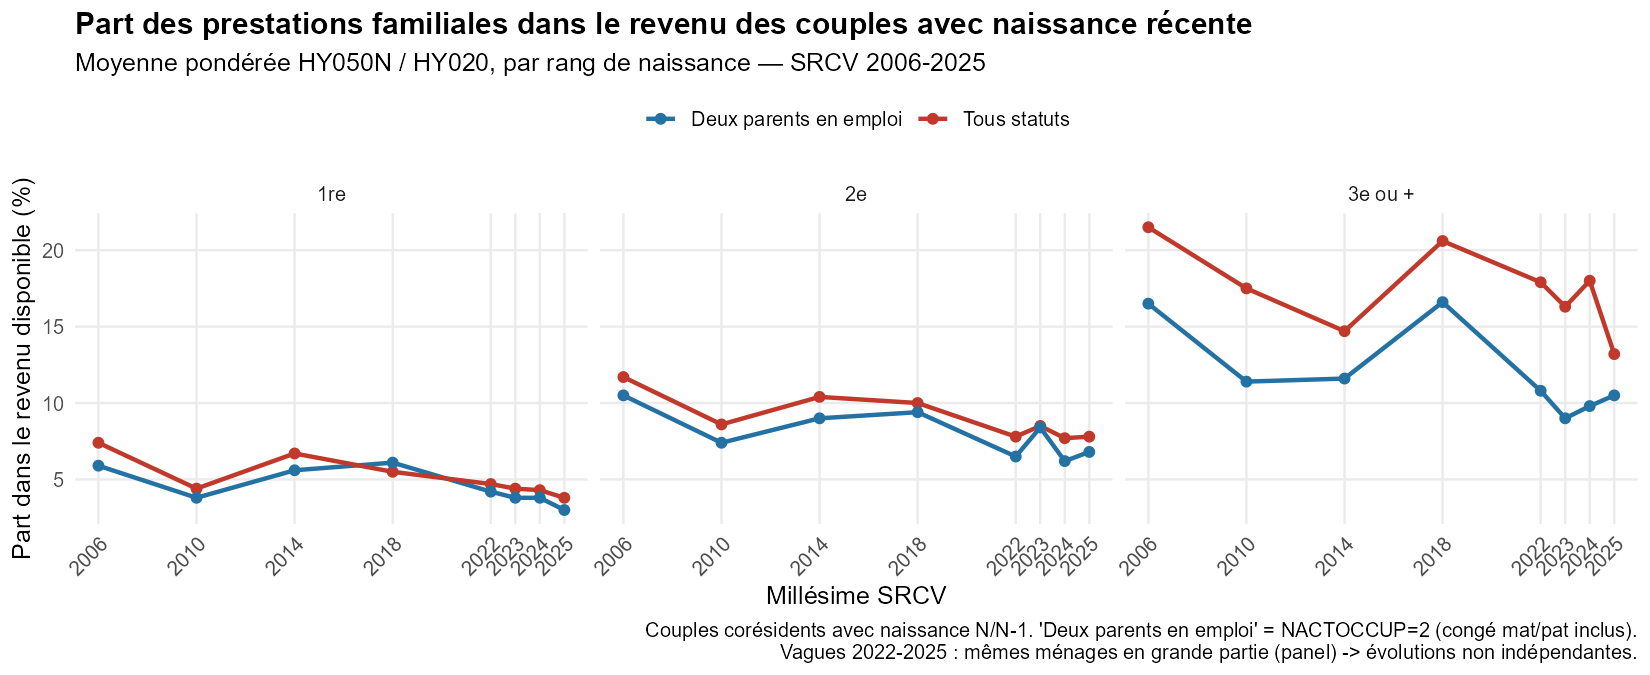
\includegraphics[width=0.95\linewidth]{part_presta_naissance}
	\caption{Part des prestations familiales dans le revenu, par rang de naissance, 2006-2025}
	\label{fig:presta}
\end{figure}

\bigskip

\noindent La lecture de cette figure demande une précaution : les vagues 2014-2018 d'une part, 2022-2025 d'autre part, interrogent en grande partie les mêmes ménages\footnote{Chaînage décrit au §\ref{sec:methode} : \texttt{DB030} identifie le même ménage à l'intérieur d'un groupe de panel (2014-2018 ; 2022-2025), mais pas d'un groupe à l'autre.} : les variations d'une vague à la suivante ne sont donc pas des tirages indépendants. La comparaison 2006-2025, elle, oppose deux vagues sans aucun chevauchement d'échantillon et reste pleinement valide.

\subsection{Le quotient familial : un avantage qui croît avec le revenu}

Le quotient familial est le miroir inversé des prestations : un avantage fiscal, dont la valeur dépend directement du montant d'impôt que le ménage aurait payé sans enfant supplémentaire — et donc de son revenu imposable. Contrairement aux prestations, il n'est diffusé dans aucune variable de SRCV : ni le nombre de parts fiscales ni le revenu imposable n'y figurent. Nous le reconstruisons donc par une micro-simulation en cinq étapes\footnote{Détail dans \texttt{R/08\_quotient\_familial.R} : (1) reconstitution des parts fiscales à partir du nombre d'enfants et de la situation de couple ; (2) approximation du revenu imposable à partir du revenu disponible, prestations non imposables retirées, abattement de 10\,\% ; (3) application du barème de l'impôt sur le revenu de l'année concernée, plafonnement du quotient familial inclus ; (4) validation contre l'impôt observé ; (5) contrefactuel retirant les parts fiscales du dernier enfant.} : nous appliquons le barème de l'impôt sur le revenu de chaque année à un revenu imposable approché, puis nous comparons l'impôt simulé avec et sans les parts fiscales du dernier enfant. L'écart est le gain de quotient familial. \\

\noindent Toute simulation fiscale doit être validée avant d'être exploitée. Comparé à l'impôt réellement déclaré par les ménages (\texttt{IRPP}), notre impôt simulé est corrélé positivement et fortement ($r = 0{,}74$), mais il le \textbf{surestime} systématiquement, de 23 à 43\,\% selon la vague, et sous-estime la part des ménages non imposables (36\,\% simulés contre 47-49\,\% observés). L'écart tient aux limites assumées de la méthode : les crédits d'impôt, la décote au-delà de son seuil d'application simplifié, et le quotient conjugal exact des pensions ne sont pas reproduits, et notre approximation du revenu imposable reste grossière faute de déclaration fiscale dans SRCV. Le niveau du gain de quotient familial que nous rapportons doit donc se lire comme un \textbf{ordre de grandeur}, pas comme un chiffrage fiscal précis ; en revanche, rien n'indique que le \textit{classement} entre ménages selon leur revenu — l'objet de notre question — soit affecté par ce biais de niveau. \\

\noindent Le champ retenu pour le contrefactuel est celui des ménages où le ménage SRCV coïncide avec le foyer fiscal\footnote{Personne de référence, conjoint marié ou pacsé le cas échéant, enfants mineurs uniquement — 76,5\,\% des ménages des quatre vagues 2022-2025. Les concubins (deux foyers fiscaux, un ménage) et les enfants majeurs (susceptibles de déclarer séparément) en sont exclus, car ils feraient apparaître dans \texttt{HY010}/\texttt{HY020} des revenus qui ne relèvent pas de la même déclaration.}, soit 11\,705 ménages avec au moins un enfant sur les quatre vagues 2022-2025. Le tableau \ref{tab:qf} présente le gain simulé par quintile de revenu brut du ménage. \\

\bigskip

\begin{table}[htbp]
	\centering
	\footnotesize
	\setlength{\tabcolsep}{6pt}
	\begin{threeparttable}
		\caption{Gain annuel de quotient familial du dernier enfant, par quintile de revenu brut du ménage}
		\label{tab:qf}
		\begin{tabular}{lrrr}
			\toprule
			Quintile & \multicolumn{1}{c}{\shortstack{Revenu brut moyen\\(k\texteuro/an)}}
			& \multicolumn{1}{c}{\shortstack{Gain moyen\\(\texteuro/an)}}
			& \multicolumn{1}{c}{\shortstack{Part sans aucun gain\\(\%)}} \\
			\midrule
			Q1 (le plus modeste) & 25,3  & 84    & 86,2 \\
			Q2                   & 45,8  & 454   & 57,8 \\
			Q3                   & 64,4  & 822   & 13,1 \\
			Q4                   & 84,4  & 1\,178 & 0,9 \\
			Q5 (le plus aisé)    & 160,6 & 1\,928 & 0,1 \\
			\bottomrule
		\end{tabular}
		\begin{tablenotes}[flushleft]\scriptsize
			\item \textit{Champ} : ménages où ménage SRCV = foyer fiscal, au moins un enfant, quatre
			vagues 2022-2025 poolées (n = 11\,705). Quintiles calculés sur le revenu brut du ménage
			(\texttt{HY010}).
			\item \textit{Lecture} : le gain fiscal moyen procuré par le dernier enfant est de
			1\,928 \texteuro/an dans le quintile de revenu le plus aisé contre 84 \texteuro/an dans le
			plus modeste, soit plus de 1\,800 \texteuro{} d'écart ; 86,2\,\% des ménages du premier
			quintile ne retirent aucun avantage du quotient familial (ménages non imposables ou dont
			l'avantage est plafonné à zéro), contre 0,1\,\% dans le dernier.
			\item \textit{Avertissement} : simulation dont le NIVEAU est surestimé (cf. texte) — à lire
			comme un ordre de grandeur, le classement entre quintiles restant l'information robuste.
			\item \textit{Source} : Insee, SRCV 2022-2025, calculs de l'auteur, barème IR officiel.
		\end{tablenotes}
	\end{threeparttable}
\end{table}

\bigskip

\noindent Le gradient est sans ambiguïté : le gain moyen passe de 84 euros par an dans le quintile le plus modeste à 1\,928 euros dans le plus aisé, un écart de plus de 1\,800 euros. Nous ne l'exprimons pas en rapport : un dénominateur aussi proche de zéro rend tout ratio instable, alors que l'écart en euros et la part des ménages sans aucun gain portent le même message sans cette fragilité. La raison n'est pas seulement que les hauts revenus sont taxés à un taux marginal plus élevé — quoique cela joue —, elle est d'abord mécanique : 86,2\,\% des ménages du premier quintile ne sont simplement pas assez imposés pour qu'une part fiscale supplémentaire leur serve à quoi que ce soit, contre 0,1\,\% dans le dernier quintile. Un instrument dont l'éligibilité dépend de l'impôt dû est par construction inopérant pour les ménages qui n'en doivent pas. \\

\noindent Le gain moyen, tous ménages avec enfant confondus, est de 880 euros par an ; il monte à 1\,476 euros parmi les seuls ménages imposables. Par rang, l'avantage est plus élevé au troisième enfant (1\,032 € en moyenne) qu'aux deux premiers (949 € et 812 €), ce qui reflète la part entière accordée à partir du troisième enfant contre une demi-part aux deux premiers — mais 51,6\,\% des ménages à leur troisième enfant n'en retirent rien du tout, contre 27,5\,\% au premier, signe que ce sont, une fois encore, des ménages différents qui accèdent à l'avantage plein. \\

\noindent Prestations et quotient familial dessinent ainsi deux logiques de redistribution inverses : les premières pèsent proportionnellement plus pour les ménages modestes, le second profite presque exclusivement aux ménages aisés. Un euro de dépense publique orienté vers l'un ou vers l'autre de ces instruments n'atteint donc pas le même ménage.

\subsection{Les mères d'un jeune enfant : qui est en emploi ?}

Le choix français de faire reposer une part de sa politique familiale sur un avantage fiscal plutôt que sur des services en nature n'est pas neutre pour l'offre de travail des mères : un avantage qui ne vaut que pour les ménages imposables incite, à la marge, à rester en emploi plutôt qu'à s'en retirer, quand un service universel de garde ne fait pas cette distinction. Nous avions annoncé, à propos de l'effet négatif et inattendu du niveau de vie sur la probabilité de naissance\footnote{Cf. §3.2 : à logement, âge et catégorie sociale donnés, les couples les plus aisés ont une probabilité de naissance plus faible.}, que le coût d'opportunité de l'interruption d'activité en était sans doute la cause. Cette dernière partie regarde directement qui, parmi les mères d'un jeune enfant, est aujourd'hui en emploi. \\

\noindent \textbf{Ce que SRCV ne permet pas de mesurer.} Il n'existe, dans les fichiers de diffusion SRCV, aucune variable de \textit{mode de garde} : ni crèche, ni assistante maternelle, ni recours aux grands-parents n'y sont renseignés\footnote{Vérifié en balayant l'intégralité des colonnes des quatre vagues FPR (2022-2025), les seules à documenter l'activité au niveau individuel.}. Nous ne pouvons donc pas chiffrer un taux de recours à la crèche, ni par le revenu ni par aucune autre variable. La variable la plus proche est \texttt{PL032}, le statut économique actuel auto-déclaré, dont une modalité isole les personnes qui se décrivent elles-mêmes comme en charge des « tâches domestiques ou de la garde d'enfants ou d'autres personnes à charge » : elle dit qui assure elle-même la garde, sans rien dire du mode de garde des autres. \\

\noindent \textbf{Champ et méthode.} Nous retenons les femmes de 18 à 45 ans, personne de référence ou conjointe, vivant avec au moins un enfant de 0 à 2 ans, sur les quatre vagues FPR 2022-2025 empilées en coupe\footnote{Une coupe, pas un panel individuel : nous n'avons pas apparié une même mère d'une vague à l'autre. L'âge du plus jeune enfant (0, 1 ou 2 ans) tient lieu d'axe temporel, en comparant des mères à des étapes différentes plutôt qu'en suivant les mêmes mères.} — soit 3\,207 observations, représentant environ 6,0 millions de mères. Une précision de vocabulaire s'impose : « en emploi » est le statut que la mère se donne elle-même (\texttt{PL032}), et une mère en congé de maternité se déclare en emploi. Les 68\,\% de mères en emploi quand l'enfant a moins d'un an ne sont donc pas des « retours » à l'emploi mais des mères qui ne l'ont pas quitté, congé compris ; nous parlerons de maintien en emploi, et non de retour. Le tableau \ref{tab:emploi_desc} présente leur statut d'activité actuel selon quatre dimensions. \\

\bigskip

\begin{table}[htbp]
	\centering
	\footnotesize
	\setlength{\tabcolsep}{5pt}
	\begin{threeparttable}
		\caption{Statut d'activité actuel des mères d'un enfant de 0 à 2 ans}
		\label{tab:emploi_desc}
		\begin{tabular}{llrrrr}
			\toprule
			& & \multicolumn{1}{c}{$n$} & \multicolumn{1}{c}{\shortstack{En emploi\\(\%)}}
			& \multicolumn{1}{c}{\shortstack{Au chômage\\(\%)}}
			& \multicolumn{1}{c}{\shortstack{Foyer / garde\\d'enfant (\%)}} \\
			\midrule
			\multirow{3}{*}{\textit{Âge du plus jeune enfant}}
			& 0 an  & 1\,150 & 68,1 & 12,1 & 14,6 \\
			& 1 an  & 1\,063 & 68,4 & 11,7 & 17,3 \\
			& 2 ans &   994  & 72,7 &  9,9 & 14,7 \\
			\addlinespace
			\multirow{5}{*}{\textit{Diplôme}}
			& Supérieur long & 1\,201 & 83,8 &  6,4 &  8,1 \\
			& Bac+2           &   507  & 77,9 & 11,4 &  5,9 \\
			& Bac              &   682  & 63,1 & 15,0 & 17,1 \\
			& CAP-BEP          &   432  & 58,7 & 14,4 & 22,1 \\
			& Infra-CAP        &   326  & 35,3 & 16,3 & 44,1 \\
			\addlinespace
			\multirow{3}{*}{\textit{Statut d'occupation du logement}}
			& Locataire                 & 1\,240 & 51,1 & 17,0 & 27,1 \\
			& Propriétaire accédant      & 1\,773 & 86,4 &  6,0 &  5,4 \\
			& Propriétaire non accédant  &   194  & 72,1 & 11,0 & 12,3 \\
			\bottomrule
		\end{tabular}
		\begin{tablenotes}[flushleft]\scriptsize
			\item \textit{Champ} : femmes de 18-45 ans, personne de référence ou conjointe, vivant avec
			au moins un enfant de 0-2 ans, France entière, vagues FPR 2022-2025 poolées en coupe.
			\item \textit{Statut d'activité} : \texttt{PL032}, statut économique actuel auto-défini ;
			« en emploi » inclut les mères en congé de maternité, qui se déclarent en emploi.
			Les modalités « incapacité de travailler », « étudiant » et « autre » ne sont pas
			reportées, d'où des lignes qui ne somment pas à 100\,\%.
			\item \textit{Lecture} : parmi les mères d'un enfant de 0-2 ans titulaires d'un diplôme
			inférieur au CAP, 35,3\,\% sont en emploi, 16,3\,\% au chômage et 44,1\,\% se déclarent en
			charge des tâches domestiques ou de la garde d'enfants.
			\item \textit{Source} : Insee, SRCV 2022-2025, calculs de l'auteur.
		\end{tablenotes}
	\end{threeparttable}
\end{table}

\bigskip

\noindent Le gradient par diplôme est le plus net des trois : 83,8\,\% des mères les plus diplômées sont en emploi contre 35,3\,\% de celles sans diplôme ou titulaires au plus du brevet, un écart de 48,5 points. Il ne se contente pas de déplacer les mères vers le chômage — le taux de chômage progresse aussi en descendant l'échelle des diplômes, mais modestement (de 6,4 à 16,3\,\%) — il les déplace surtout vers le foyer : 44,1\,\% des mères les moins diplômées se déclarent elles-mêmes en charge de la garde de leur enfant, contre 8,1\,\% des plus diplômées. L'écart par statut de logement est tout aussi marqué (51,1\,\% en emploi chez les locataires contre 86,4\,\% chez les accédants), mais il faut se garder d'y lire un effet du logement sur l'emploi : la causalité la plus plausible va en sens inverse, un revenu stable et un emploi étant des conditions quasi nécessaires à l'accession à la propriété. Nous y revenons plus bas. \\

\noindent Le tableau \ref{tab:emploi_modele} reprend ces trois dimensions dans un modèle unique, qui permet de savoir ce qui reste une fois les autres facteurs pris en compte. \\

\bigskip

\begin{table}[htbp]
	\centering
	\footnotesize
	\setlength{\tabcolsep}{5pt}
	\begin{threeparttable}
		\caption{Probabilité d'être en emploi pour une mère d'un enfant de 0-2 ans (effets marginaux moyens, points de pourcentage)}
		\label{tab:emploi_modele}
		\begin{tabular}{lrrr}
			\toprule
			Variable & \multicolumn{1}{c}{Effet} & \multicolumn{2}{c}{IC à 95\,\%} \\
			\midrule
			\multicolumn{4}{l}{\textit{Âge du plus jeune enfant (réf. 0 an)}} \\
			\quad 1 an  & $-0{,}6$          & [$-4{,}6$ & $3{,}4$]  \\
			\quad 2 ans & $+2{,}8$          & [$-1{,}3$ & $7{,}0$]  \\
			\addlinespace
			\multicolumn{4}{l}{\textit{Diplôme (réf. Bac)}} \\
			\quad Bac+2            & $+8{,}0$\sym{*}   & [$0{,}7$  & $15{,}2$] \\
			\quad CAP-BEP          & $-0{,}3$          & [$-7{,}8$ & $7{,}2$]  \\
			\quad Infra-CAP        & $-14{,}9$\sym{**} & [$-23{,}8$ & $-6{,}1$] \\
			\quad Supérieur long   & $+13{,}1$\sym{***} & [$6{,}7$  & $19{,}5$] \\
			\addlinespace
			\multicolumn{4}{l}{\textit{Statut de logement (réf. Locataire)}} \\
			\quad Propriétaire accédant     & $+23{,}2$\sym{***} & [$17{,}9$ & $28{,}6$] \\
			\quad Propriétaire non accédant & $+12{,}9$\sym{**}  & [$4{,}0$  & $21{,}8$] \\
			\addlinespace
			\midrule
			Observations & \multicolumn{3}{r}{3\,148} \\
			En emploi & \multicolumn{3}{r}{2\,285} \\
			\bottomrule
		\end{tabular}
		\begin{tablenotes}[flushleft]\scriptsize
			\item \sym{***} $p<0{,}001$ ; \sym{**} $p<0{,}01$ ; \sym{*} $p<0{,}05$.
			\item \textit{Champ} : identique au tableau \ref{tab:emploi_desc}, diplôme renseigné.
			\item \textit{Modèle} : probit pondéré (poids \texttt{RB050}), erreurs-types regroupées par
			individu, effets fixes d'année. Contrôles additionnels : nombre d'enfants du ménage, âge de
			la mère, degré d'urbanisation, ZEAT. Le niveau de vie du ménage n'est volontairement PAS
			contrôlé : il intègre le salaire de la mère elle-même, ce qui en ferait un contrôle de
			l'issue par elle-même.
			\item \textit{Lecture} : à caractéristiques égales, une mère titulaire d'un diplôme
			inférieur au CAP a une probabilité d'être en emploi inférieure de 14,9 points à une mère
			bachelière, sur un taux de référence proche de 73\,\% (part en emploi dans le champ complet).
			\item \textit{Source} : Insee, SRCV 2022-2025, calculs de l'auteur.
		\end{tablenotes}
	\end{threeparttable}
\end{table}

\bigskip

\noindent Trois lectures s'imposent. L'\textbf{âge de l'enfant}, une fois les autres facteurs pris en compte, ne joue plus : l'écart brut entre 0 et 2 ans (68,1\,\% contre 72,7\,\% dans le tableau \ref{tab:emploi_desc}) était pour l'essentiel un effet de composition, absorbé ici par le diplôme et le rang. Le \textbf{diplôme}, lui, résiste entièrement au contrôle et reste le facteur le plus puissant du modèle : l'écart entre le bas et le haut de l'échelle atteint 28 points (de $-14{,}9$ à $+13{,}1$ par rapport au bac). C'est la confirmation directe de l'intuition avancée au §3.2 — le coût d'opportunité d'interrompre une carrière qualifiée est élevé, celui d'interrompre un emploi peu qualifié beaucoup moins, et c'est ce différentiel, plus que l'âge de l'enfant, qui organise le maintien en emploi. \\

\noindent Le \textbf{statut de logement}, enfin, porte l'effet le plus large du modèle : 23,2 points entre propriétaires accédants et locataires, à diplôme, âge et rang égaux. Nous ne le lisons pas comme un effet causal du logement sur l'emploi maternel — aucun dispositif de ce travail ne permet de l'établir dans ce sens, et la lecture inverse est plus économique : un couple accède à la propriété parce qu'il dispose d'un revenu stable, ce qui suppose le plus souvent que les deux conjoints travaillent, l'octroi d'un crédit immobilier reposant largement sur la pérennité des revenus du ménage. L'écart mesure ainsi, pour une bonne part, une sélection plutôt qu'un effet du logement lui-même — à la différence de l'effet de la surface sur la première naissance au §3.2, nous ne disposons ici d'aucun équivalent du test des non-déménageurs pour trancher. \\

\noindent Un dernier résultat, purement descriptif, mérite d'être noté : parmi les mères dont le calendrier d'activité de l'année précédente indique un congé maternité ou paternité d'au moins six mois, 75,6\,\% sont en emploi aujourd'hui ; parmi celles qui étaient déjà, l'année précédente, six mois ou plus au foyer, seules 8,0\,\% le sont\footnote{Lecture prudente : ces deux catégories ne sont pas symétriques, la seconde inclut par construction des mères déjà installées dans l'inactivité avant même la naissance récente, la comparaison mesure autant une persistance d'état qu'un retour à l'emploi proprement dit.}. Le congé, en lui-même, ne semble donc pas être la porte de sortie de l'emploi : c'est l'installation dans l'inactivité, quand elle survient, qui tend à se prolonger.

\bigskip

\noindent En résumé, les trois instruments examinés dans cette partie racontent la même histoire sous trois angles différents. Les prestations en espèces redistribuent, mais leur poids s'est effrité de moitié en vingt ans pour les familles nombreuses. Le quotient familial, lui, profite presque exclusivement aux ménages déjà aisés, par construction. Et le maintien en emploi des mères, sur lequel repose une partie de la valeur de cet avantage fiscal, se joue d'abord sur le diplôme — c'est-à-dire sur le coût d'opportunité de l'interruption — bien davantage que sur l'âge de l'enfant. Une politique familiale qui privilégie l'avantage fiscal à la place du service en nature aide, par construction, les ménages qui en ont le moins besoin pour travailler, et laisse de côté ceux pour qui la reprise d'un emploi est la moins évidente.
	
	\section{Conclusion}
	
	Cette étude est partie d'une question simple, le logement pèse-t-il sur la natalité, et d'une conviction, que la réponse devait être cherchée au niveau du couple et de sa décision. Trois enseignements se dégagent. \\

\noindent Le premier est que le débat public est mal posé lorsqu'il parle de prix. À revenu et à prix au mètre carré donnés, le coût du logement n'a aucun effet sur la probabilité d'une naissance ; la surface en a un, et il ne prend pas la forme que l'on attendrait. Ce n'est pas « plus c'est grand, plus on fait d'enfants », c'est « en dessous d'une soixantaine de mètres carrés, on ne fonde pas de famille ». Ce seuil concerne le premier enfant, il est estimé et non posé, et il est d'autant plus marqué que le marché est tendu. Sa conséquence pratique est que la surface moyenne des logements est un mauvais indicateur : elle n'a pas bougé en quinze ans pendant que la part des couples sans enfant logés sous le seuil gagnait trois à quatre points. Il faut cependant le dire aussi nettement : cette association n'est probablement pas causale. Sur les mêmes ménages, la surface est liée à la naissance qui vient d'avoir lieu et ne prédit pas celle qui suit, ce qui est la signature d'un logement choisi pour un projet de famille plutôt que d'une contrainte qui l'empêcherait. \\

\noindent Le deuxième est que le logement, ainsi mesuré, n'explique pas la baisse de la fécondité française depuis 2010 — ou plutôt qu'il l'explique par un canal et la compense par un autre. La dégradation par le bas de la distribution des surfaces aurait, seule, retiré entre un vingtième et un dixième de la baisse ; la progression de l'accession à la propriété, permise par quinze ans de taux d'intérêt bas, en a rendu autant. Le solde est nul, et sa borne haute, si l'on refuse de croire à l'effet compensateur de l'accession, est d'un dixième. Mais ce solde est nul pour une raison conjoncturelle qui n'a aucune vocation à se reproduire : les taux sont remontés, et si le canal favorable s'éteint pendant que celui des petites surfaces continue de jouer, la période qui s'ouvre ne ressemblera pas à celle que nous avons mesurée. Il faut aussi rappeler ce que ce chiffre ne couvre pas : les couples qui ne se forment pas, ou plus tard, faute de pouvoir se loger, canal que nos données ne voient pas et où le logement joue peut-être le plus. \\

\noindent Le troisième porte sur la politique familiale. Ses trois instruments ne s'adressent pas aux mêmes ménages : les prestations en espèces vont d'abord aux familles nombreuses, mais leur poids a fondu de moitié en vingt ans ; le quotient familial va presque exclusivement aux ménages aisés, par construction ; et le maintien en emploi des mères d'un jeune enfant se décide sur le diplôme, c'est-à-dire sur le coût d'opportunité de l'interruption, davantage que sur l'âge de l'enfant. Un pays qui consacre un quart de sa dépense familiale à des exonérations fiscales soutient, à la marge, les mères pour qui rester en emploi est déjà le choix le plus naturel, et laisse sans levier celles pour qui il ne l'est pas. \\

\noindent Plusieurs prolongements s'imposent. Le premier est d'identification : seul un dispositif exploitant une variation exogène de l'offre de logements — un programme de construction, une réforme locale du zonage — permettrait de trancher entre contrainte et préférence. Le deuxième est de champ : mesurer l'effet du logement sur la formation des couples et l'âge à la décohabitation, là où nos données sont muettes. Le troisième est de données : les fichiers SRCV ne portent aucune variable de mode de garde, ce qui interdit de mesurer directement ce que la crèche fait à l'emploi des mères, alors que c'est le paramètre le plus discuté de la politique familiale ; et la naissance y est reconstruite depuis 2022 d'une façon qui compte deux fois la moitié des enfants, ce qui appelle le retour d'un module « événements » dans les fichiers de recherche. Enfin, l'anomalie de pondération des vagues 2022 et 2023 que nous documentons en annexe mérite d'être signalée aux producteurs de l'enquête, car elle affecte précisément les ménages avec nouveau-né, c'est-à-dire l'objet même de cette étude.
	
	\section*{Bibliographie}
	\addcontentsline{toc}{section}{Bibliographie}
	\markboth{Bibliographie}{}
	
	\begin{itemize}[leftmargin=1.2em]
		\item Assemblée nationale (2026), \textit{Rapport d’information n\textsuperscript{o} 2474 fait au nom de la mission d’information sur les causes et conséquences de la baisse de la natalité en France}, présidente C. de Pélichy, rapporteur J. Patrier-Leitus, déposé le 11 février 2026.
		\item Couillard B. K. (2025), « Build, Baby, Build: How Housing Shapes Fertility », document de travail, University of Toronto.
		\item Debest C., Mazuy M. (2014), « Rester sans enfant : un choix de vie à contre-courant », \textit{Population \& Sociétés}, n\textsuperscript{o} 508, Ined.
		\item Dettling L. J., Kearney M. S. (2014), « House Prices and Birth Rates: The Impact of the Real Estate Market on the Decision to Have a Baby », \textit{Journal of Public Economics}, vol. 110, p. 82-100.
		\item Doepke M., Hannusch A., Kindermann F., Tertilt M. (2023), « The Economics of Fertility: A New Era », in \textit{Handbook of the Economics of the Family}, vol. 1, Elsevier, p. 151-254.
		\item Insee (2020), « Les femmes les plus modestes et les plus aisées ont le plus d’enfants », \textit{Insee Première}, n\textsuperscript{o} 1826.
		\item Insee (2022), « Fécondité selon le niveau de vie : une nouvelle estimation », \textit{Insee Analyses}, n\textsuperscript{o} 72.
		\item Insee (2026), « Bilan démographique 2025 », \textit{Insee Première}, n\textsuperscript{o} 2087, février 2026.
		\item MeilleursAgents (2022), « Le pouvoir d’achat immobilier en baisse dans les grandes villes », Baromètre MeilleursAgents.
		\item Saudubray (2026), référence complète à fournir par l’auteur.
	\end{itemize}

\newpage

	\appendix
	
	\section{Evolution du prix et des surfaces des logements chez les 20-39 ans}\label{annexe1}
	
	Dans cette section Nous présentons les chiffres détaillés sur les conditions de logement moyennes des jeunes en France, en fonction de leur statut de locataire ou de propriétaire accédant. Nous ne proposons pas les propriétaires non accédants et les personnes logées à titre gratuit car elles sont marginales dans les données et que nous préférons nous focaliser sur les ménages avec des dépenses mensuelles plus élevées. Dans les deux sous-parties suivantes nous présentons les résultats en déflatant par les prix (l'indice des prix à la consommation de 2006 à 2025) puis par les revenus, en rapportant les évolutions du prix aux évolutions du revenu, et en proposant ainsi un taux d'effort moyen représentant la part des dépenses de logement dans le revenu. 
	
	\subsection{Prix déflatés de l'inflation}\label{annexe1a}
	
	Les quatre tableaux ci-après présentent les variations des surfaces, prix et prix au m$^2$ pour les quatre classes d'âge retenues, le tout déflaté de l'indice des prix à la consommation. 
	
	\begin{table}[htbp]
		\centering
		\footnotesize
		\setlength{\tabcolsep}{4pt}
		\begin{threeparttable}
			\caption{Conditions de logement des ménages dont la personne de référence a 20-24 ans (coûts en euros constants de 2025)}
			\label{tab:logementipc_20_24}
			\begin{tabular}{lrrrrrrrr}
				\toprule
				& \multicolumn{4}{c}{Locataires} & \multicolumn{4}{c}{Propriétaires accédants} \\
				\cmidrule(lr){2-5} \cmidrule(lr){6-9}
				Année & \multicolumn{1}{c}{\shortstack{Surface\\(m\textsuperscript{2})}} & \multicolumn{1}{c}{\shortstack{Coût\\(\texteuro/mois)}} & \multicolumn{1}{c}{\shortstack{Coût/m\textsuperscript{2}\\(\texteuro)}} & \multicolumn{1}{c}{\shortstack{\textit{n}}} & \multicolumn{1}{c}{\shortstack{Surface\\(m\textsuperscript{2})}} & \multicolumn{1}{c}{\shortstack{Coût\\(\texteuro/mois)}} & \multicolumn{1}{c}{\shortstack{Coût/m\textsuperscript{2}\\(\texteuro)}} & \multicolumn{1}{c}{\shortstack{\textit{n}}} \\
				\midrule
				2006 & 56,6 & 670 & 13,8 & {\scriptsize 264} & --- & --- & --- & {\scriptsize 23} \\
				2010 & 54,2 & 707 & 15,5 & {\scriptsize 274} & --- & --- & --- & {\scriptsize 9} \\
				2014 & 52,9 & 712 & 16,1 & {\scriptsize 212} & --- & --- & --- & {\scriptsize 12} \\
				2018 & 50,0 & 689 & 16,8 & {\scriptsize 206} & --- & --- & --- & {\scriptsize 12} \\
				\addlinespace
				2022 & 49,8 & 698 & 17,0 & {\scriptsize 239} & --- & --- & --- & {\scriptsize 17} \\
				2023 & 49,8 & 639 & 16,5 & {\scriptsize 204} & --- & --- & --- & {\scriptsize 19} \\
				2024 & 50,9 & 715 & 16,8 & {\scriptsize 224} & --- & --- & --- & {\scriptsize 23} \\
				2025 & 51,7 & 745 & 17,4 & {\scriptsize 219} & --- & --- & --- & {\scriptsize 13} \\
				\bottomrule
			\end{tabular}
			\begin{tablenotes}[flushleft]\scriptsize
				\item \textit{Champ} : ménages dont la personne de référence a 20-24 ans, France entière.
				\item \textit{Lecture} : moyennes pondérées (poids de sondage SRCV). Coût du logement =
				charges (\texttt{HH070}) + mensualité de remboursement (\texttt{REMP}/\texttt{REMPR}).
				\item \textit{Déflateur} : coûts déflatés par l'indice des prix à la consommation (Insee, base 100 = 2025) ; les montants sont en euros de pouvoir d'achat constant.
				\item \textit{n} : effectif non pondéré de la cellule. Les moyennes reposant sur
				moins de 30 observations ne sont pas reportées et sont remplacées par ---.
				\item \textit{Source} : Insee, SRCV 2006-2025, calculs de l'auteur.
			\end{tablenotes}
		\end{threeparttable}
	\end{table}
	
	\begin{table}[htbp]
		\centering
		\footnotesize
		\setlength{\tabcolsep}{4pt}
		\begin{threeparttable}
			\caption{Conditions de logement des ménages dont la personne de référence a 25-29 ans (coûts en euros constants de 2025)}
			\label{tab:logementipc_25_29}
			\begin{tabular}{lrrrrrrrr}
				\toprule
				& \multicolumn{4}{c}{Locataires} & \multicolumn{4}{c}{Propriétaires accédants} \\
				\cmidrule(lr){2-5} \cmidrule(lr){6-9}
				Année & \multicolumn{1}{c}{\shortstack{Surface\\(m\textsuperscript{2})}} & \multicolumn{1}{c}{\shortstack{Coût\\(\texteuro/mois)}} & \multicolumn{1}{c}{\shortstack{Coût/m\textsuperscript{2}\\(\texteuro)}} & \multicolumn{1}{c}{\shortstack{\textit{n}}} & \multicolumn{1}{c}{\shortstack{Surface\\(m\textsuperscript{2})}} & \multicolumn{1}{c}{\shortstack{Coût\\(\texteuro/mois)}} & \multicolumn{1}{c}{\shortstack{Coût/m\textsuperscript{2}\\(\texteuro)}} & \multicolumn{1}{c}{\shortstack{\textit{n}}} \\
				\midrule
				2006 & 60,3 & 734 & 13,8 & {\scriptsize 404} & 83,9 & 1\,531 & 20,8 & {\scriptsize 103} \\
				2010 & 62,7 & 779 & 14,2 & {\scriptsize 406} & 86,8 & 1\,638 & 21,2 & {\scriptsize 166} \\
				2014 & 61,6 & 824 & 15,1 & {\scriptsize 385} & 93,4 & 1\,547 & 19,4 & {\scriptsize 137} \\
				2018 & 61,6 & 756 & 15,1 & {\scriptsize 337} & 91,5 & 1\,300 & 15,7 & {\scriptsize 118} \\
				\addlinespace
				2022 & 55,9 & 766 & 16,2 & {\scriptsize 378} & 89,9 & 1\,200 & 15,5 & {\scriptsize 166} \\
				2023 & 56,4 & 774 & 15,5 & {\scriptsize 349} & 91,5 & 1\,206 & 15,0 & {\scriptsize 159} \\
				2024 & 61,5 & 801 & 14,8 & {\scriptsize 358} & 86,4 & 1\,298 & 17,0 & {\scriptsize 171} \\
				2025 & 58,4 & 788 & 15,8 & {\scriptsize 336} & 90,0 & 1\,439 & 17,7 & {\scriptsize 154} \\
				\bottomrule
			\end{tabular}
			\begin{tablenotes}[flushleft]\scriptsize
				\item \textit{Champ} : ménages dont la personne de référence a 25-29 ans, France entière.
				\item \textit{Lecture} : moyennes pondérées (poids de sondage SRCV). Coût du logement =
				charges (\texttt{HH070}) + mensualité de remboursement (\texttt{REMP}/\texttt{REMPR}).
				\item \textit{Déflateur} : coûts déflatés par l'indice des prix à la consommation (Insee, base 100 = 2025) ; les montants sont en euros de pouvoir d'achat constant.
				\item \textit{n} : effectif non pondéré de la cellule. Les moyennes reposant sur
				moins de 30 observations ne sont pas reportées et sont remplacées par ---.
				\item \textit{Source} : Insee, SRCV 2006-2025, calculs de l'auteur.
			\end{tablenotes}
		\end{threeparttable}
	\end{table}
	
	\begin{table}[htbp]
		\centering
		\footnotesize
		\setlength{\tabcolsep}{4pt}
		\begin{threeparttable}
			\caption{Conditions de logement des ménages dont la personne de référence a 30-34 ans (coûts en euros constants de 2025)}
			\label{tab:logementipc_30_34}
			\begin{tabular}{lrrrrrrrr}
				\toprule
				& \multicolumn{4}{c}{Locataires} & \multicolumn{4}{c}{Propriétaires accédants} \\
				\cmidrule(lr){2-5} \cmidrule(lr){6-9}
				Année & \multicolumn{1}{c}{\shortstack{Surface\\(m\textsuperscript{2})}} & \multicolumn{1}{c}{\shortstack{Coût\\(\texteuro/mois)}} & \multicolumn{1}{c}{\shortstack{Coût/m\textsuperscript{2}\\(\texteuro)}} & \multicolumn{1}{c}{\shortstack{\textit{n}}} & \multicolumn{1}{c}{\shortstack{Surface\\(m\textsuperscript{2})}} & \multicolumn{1}{c}{\shortstack{Coût\\(\texteuro/mois)}} & \multicolumn{1}{c}{\shortstack{Coût/m\textsuperscript{2}\\(\texteuro)}} & \multicolumn{1}{c}{\shortstack{\textit{n}}} \\
				\midrule
				2006 & 69,5 & 789 & 13,5 & {\scriptsize 377} & 105,3 & 1\,639 & 17,2 & {\scriptsize 337} \\
				2010 & 69,5 & 836 & 13,8 & {\scriptsize 365} & 98,0 & 1\,716 & 20,2 & {\scriptsize 322} \\
				2014 & 64,5 & 835 & 14,8 & {\scriptsize 325} & 103,6 & 1\,754 & 18,7 & {\scriptsize 314} \\
				2018 & 66,4 & 801 & 13,7 & {\scriptsize 326} & 100,7 & 1\,567 & 17,6 & {\scriptsize 278} \\
				\addlinespace
				2022 & 63,2 & 809 & 14,8 & {\scriptsize 449} & 105,3 & 1\,508 & 16,5 & {\scriptsize 386} \\
				2023 & 62,6 & 818 & 15,0 & {\scriptsize 397} & 102,0 & 1\,462 & 16,7 & {\scriptsize 361} \\
				2024 & 60,7 & 850 & 16,2 & {\scriptsize 395} & 103,0 & 1\,495 & 17,1 & {\scriptsize 380} \\
				2025 & 61,1 & 874 & 16,5 & {\scriptsize 422} & 103,5 & 1\,464 & 17,1 & {\scriptsize 377} \\
				\bottomrule
			\end{tabular}
			\begin{tablenotes}[flushleft]\scriptsize
				\item \textit{Champ} : ménages dont la personne de référence a 30-34 ans, France entière.
				\item \textit{Lecture} : moyennes pondérées (poids de sondage SRCV). Coût du logement =
				charges (\texttt{HH070}) + mensualité de remboursement (\texttt{REMP}/\texttt{REMPR}).
				\item \textit{Déflateur} : coûts déflatés par l'indice des prix à la consommation (Insee, base 100 = 2025) ; les montants sont en euros de pouvoir d'achat constant.
				\item \textit{n} : effectif non pondéré de la cellule. Les moyennes reposant sur
				moins de 30 observations ne sont pas reportées et sont remplacées par ---.
				\item \textit{Source} : Insee, SRCV 2006-2025, calculs de l'auteur.
			\end{tablenotes}
		\end{threeparttable}
	\end{table}
	
	\begin{table}[htbp]
		\centering
		\footnotesize
		\setlength{\tabcolsep}{4pt}
		\begin{threeparttable}
			\caption{Conditions de logement des ménages dont la personne de référence a 35-39 ans (coûts en euros constants de 2025)}
			\label{tab:logementipc_35_39}
			\begin{tabular}{lrrrrrrrr}
				\toprule
				& \multicolumn{4}{c}{Locataires} & \multicolumn{4}{c}{Propriétaires accédants} \\
				\cmidrule(lr){2-5} \cmidrule(lr){6-9}
				Année & \multicolumn{1}{c}{\shortstack{Surface\\(m\textsuperscript{2})}} & \multicolumn{1}{c}{\shortstack{Coût\\(\texteuro/mois)}} & \multicolumn{1}{c}{\shortstack{Coût/m\textsuperscript{2}\\(\texteuro)}} & \multicolumn{1}{c}{\shortstack{\textit{n}}} & \multicolumn{1}{c}{\shortstack{Surface\\(m\textsuperscript{2})}} & \multicolumn{1}{c}{\shortstack{Coût\\(\texteuro/mois)}} & \multicolumn{1}{c}{\shortstack{Coût/m\textsuperscript{2}\\(\texteuro)}} & \multicolumn{1}{c}{\shortstack{\textit{n}}} \\
				\midrule
				2006 & 72,3 & 813 & 12,4 & {\scriptsize 388} & 109,3 & 1\,781 & 17,4 & {\scriptsize 471} \\
				2010 & 72,2 & 854 & 13,1 & {\scriptsize 392} & 110,7 & 1\,746 & 17,8 & {\scriptsize 500} \\
				2014 & 71,5 & 909 & 14,4 & {\scriptsize 343} & 105,4 & 1\,681 & 17,2 & {\scriptsize 511} \\
				2018 & 73,2 & 838 & 13,0 & {\scriptsize 306} & 106,6 & 1\,694 & 17,9 & {\scriptsize 383} \\
				\addlinespace
				2022 & 67,1 & 867 & 14,4 & {\scriptsize 435} & 108,2 & 1\,637 & 17,6 & {\scriptsize 630} \\
				2023 & 70,0 & 826 & 13,4 & {\scriptsize 408} & 105,9 & 1\,517 & 16,3 & {\scriptsize 575} \\
				2024 & 69,4 & 844 & 13,5 & {\scriptsize 413} & 107,0 & 1\,656 & 17,3 & {\scriptsize 616} \\
				2025 & 65,4 & 895 & 15,4 & {\scriptsize 443} & 107,7 & 1\,796 & 19,5 & {\scriptsize 608} \\
				\bottomrule
			\end{tabular}
			\begin{tablenotes}[flushleft]\scriptsize
				\item \textit{Champ} : ménages dont la personne de référence a 35-39 ans, France entière.
				\item \textit{Lecture} : moyennes pondérées (poids de sondage SRCV). Coût du logement =
				charges (\texttt{HH070}) + mensualité de remboursement (\texttt{REMP}/\texttt{REMPR}).
				\item \textit{Déflateur} : coûts déflatés par l'indice des prix à la consommation (Insee, base 100 = 2025) ; les montants sont en euros de pouvoir d'achat constant.
				\item \textit{n} : effectif non pondéré de la cellule. Les moyennes reposant sur
				moins de 30 observations ne sont pas reportées et sont remplacées par ---.
				\item \textit{Source} : Insee, SRCV 2006-2025, calculs de l'auteur.
			\end{tablenotes}
		\end{threeparttable}
	\end{table}

\newpage

\subsection{prix déflatés du revenu }\label{annexe1b}

\begin{table}[htbp]
	\centering
	\footnotesize
	\setlength{\tabcolsep}{4pt}
	\begin{threeparttable}
		\caption{Conditions de logement des ménages dont la personne de référence a 20-24 ans}
		\label{tab:logement_20_24}
		\begin{tabular}{lrrrrrrrrrr}
			\toprule
			& \multicolumn{5}{c}{Locataires} & \multicolumn{5}{c}{Propriétaires accédants} \\
			\cmidrule(lr){2-6} \cmidrule(lr){7-11}
			Année & \multicolumn{1}{c}{\shortstack{Surface\\(m\textsuperscript{2})}} & \multicolumn{1}{c}{\shortstack{Coût\\(\texteuro/mois)}} & \multicolumn{1}{c}{\shortstack{Coût/m\textsuperscript{2}\\(\texteuro)}} & \multicolumn{1}{c}{\shortstack{Effort\\(\%)}} & \multicolumn{1}{c}{\shortstack{\textit{n}}} & \multicolumn{1}{c}{\shortstack{Surface\\(m\textsuperscript{2})}} & \multicolumn{1}{c}{\shortstack{Coût\\(\texteuro/mois)}} & \multicolumn{1}{c}{\shortstack{Coût/m\textsuperscript{2}\\(\texteuro)}} & \multicolumn{1}{c}{\shortstack{Effort\\(\%)}} & \multicolumn{1}{c}{\shortstack{\textit{n}}} \\
			\midrule
			2006 & 56,6 & 823 & 17,0 & 44,0 & {\scriptsize 264} & --- & --- & --- & --- & {\scriptsize 23} \\
			2010 & 54,2 & 737 & 16,1 & 48,2 & {\scriptsize 274} & --- & --- & --- & --- & {\scriptsize 9} \\
			2014 & 52,9 & 733 & 16,6 & 48,3 & {\scriptsize 212} & --- & --- & --- & --- & {\scriptsize 12} \\
			2018 & 50,0 & 695 & 16,9 & 45,0 & {\scriptsize 206} & --- & --- & --- & --- & {\scriptsize 12} \\
			\addlinespace
			2022 & 49,8 & 746 & 18,2 & 49,2 & {\scriptsize 239} & --- & --- & --- & --- & {\scriptsize 17} \\
			2023 & 49,8 & 680 & 17,6 & 45,2 & {\scriptsize 204} & --- & --- & --- & --- & {\scriptsize 19} \\
			2024 & 50,9 & 736 & 17,3 & 41,8 & {\scriptsize 224} & --- & --- & --- & --- & {\scriptsize 23} \\
			2025 & 51,7 & 745 & 17,4 & 46,7 & {\scriptsize 219} & --- & --- & --- & --- & {\scriptsize 13} \\
			\bottomrule
		\end{tabular}
		\begin{tablenotes}[flushleft]\scriptsize
			\item \textit{Champ} : ménages dont la personne de référence a 20-24 ans, France entière.
			\item \textit{Lecture} : moyennes pondérées (poids de sondage SRCV). Coût du logement =
			charges (\texttt{HH070}) + mensualité de remboursement (\texttt{REMP}/\texttt{REMPR}).
			Taux d'effort = coût annuel rapporté au revenu disponible, borné à [0 ; 100]\,\%.
			\item \textit{Déflateur} : coûts déflatés par l'indice du niveau de vie médian de chaque vague (base 100 = 2025) ; un montant stable signifie une progression au même rythme que les revenus.
			\item \textit{n} : effectif non pondéré de la cellule. Les moyennes reposant sur
			moins de 30 observations ne sont pas reportées et sont remplacées par ---.
			\item \textit{Source} : Insee, SRCV 2006-2025, calculs de l'auteur.
		\end{tablenotes}
	\end{threeparttable}
\end{table}

\begin{table}[htbp]
	\centering
	\footnotesize
	\setlength{\tabcolsep}{4pt}
	\begin{threeparttable}
		\caption{Conditions de logement des ménages dont la personne de référence a 25-29 ans}
		\label{tab:logement_25_29}
		\begin{tabular}{lrrrrrrrrrr}
			\toprule
			& \multicolumn{5}{c}{Locataires} & \multicolumn{5}{c}{Propriétaires accédants} \\
			\cmidrule(lr){2-6} \cmidrule(lr){7-11}
			Année & \multicolumn{1}{c}{\shortstack{Surface\\(m\textsuperscript{2})}} & \multicolumn{1}{c}{\shortstack{Coût\\(\texteuro/mois)}} & \multicolumn{1}{c}{\shortstack{Coût/m\textsuperscript{2}\\(\texteuro)}} & \multicolumn{1}{c}{\shortstack{Effort\\(\%)}} & \multicolumn{1}{c}{\shortstack{\textit{n}}} & \multicolumn{1}{c}{\shortstack{Surface\\(m\textsuperscript{2})}} & \multicolumn{1}{c}{\shortstack{Coût\\(\texteuro/mois)}} & \multicolumn{1}{c}{\shortstack{Coût/m\textsuperscript{2}\\(\texteuro)}} & \multicolumn{1}{c}{\shortstack{Effort\\(\%)}} & \multicolumn{1}{c}{\shortstack{\textit{n}}} \\
			\midrule
			2006 & 60,3 & 900 & 17,0 & 33,8 & {\scriptsize 404} & 83,9 & 1\,879 & 25,6 & 44,9 & {\scriptsize 103} \\
			2010 & 62,7 & 812 & 14,8 & 36,5 & {\scriptsize 406} & 86,8 & 1\,709 & 22,1 & 43,7 & {\scriptsize 166} \\
			2014 & 61,6 & 849 & 15,5 & 34,8 & {\scriptsize 385} & 93,4 & 1\,593 & 20,0 & 43,0 & {\scriptsize 137} \\
			2018 & 61,6 & 762 & 15,2 & 32,0 & {\scriptsize 337} & 91,5 & 1\,311 & 15,9 & 36,9 & {\scriptsize 118} \\
			\addlinespace
			2022 & 55,9 & 818 & 17,3 & 35,0 & {\scriptsize 378} & 89,9 & 1\,283 & 16,6 & 36,9 & {\scriptsize 166} \\
			2023 & 56,4 & 823 & 16,5 & 32,6 & {\scriptsize 349} & 91,5 & 1\,284 & 15,9 & 34,3 & {\scriptsize 159} \\
			2024 & 61,5 & 824 & 15,3 & 31,3 & {\scriptsize 358} & 86,4 & 1\,335 & 17,5 & 35,0 & {\scriptsize 171} \\
			2025 & 58,4 & 788 & 15,8 & 31,6 & {\scriptsize 336} & 90,0 & 1\,439 & 17,7 & 37,5 & {\scriptsize 154} \\
			\bottomrule
		\end{tabular}
		\begin{tablenotes}[flushleft]\scriptsize
			\item \textit{Champ} : ménages dont la personne de référence a 25-29 ans, France entière.
			\item \textit{Lecture} : moyennes pondérées (poids de sondage SRCV). Coût du logement =
			charges (\texttt{HH070}) + mensualité de remboursement (\texttt{REMP}/\texttt{REMPR}).
			Taux d'effort = coût annuel rapporté au revenu disponible, borné à [0 ; 100]\,\%.
			\item \textit{Déflateur} : coûts déflatés par l'indice du niveau de vie médian de chaque vague (base 100 = 2025) ; un montant stable signifie une progression au même rythme que les revenus.
			\item \textit{n} : effectif non pondéré de la cellule. Les moyennes reposant sur
			moins de 30 observations ne sont pas reportées et sont remplacées par ---.
			\item \textit{Source} : Insee, SRCV 2006-2025, calculs de l'auteur.
		\end{tablenotes}
	\end{threeparttable}
\end{table}

\begin{table}[htbp]
	\centering
	\footnotesize
	\setlength{\tabcolsep}{4pt}
	\begin{threeparttable}
		\caption{Conditions de logement des ménages dont la personne de référence a 30-34 ans}
		\label{tab:logement_30_34}
		\begin{tabular}{lrrrrrrrrrr}
			\toprule
			& \multicolumn{5}{c}{Locataires} & \multicolumn{5}{c}{Propriétaires accédants} \\
			\cmidrule(lr){2-6} \cmidrule(lr){7-11}
			Année & \multicolumn{1}{c}{\shortstack{Surface\\(m\textsuperscript{2})}} & \multicolumn{1}{c}{\shortstack{Coût\\(\texteuro/mois)}} & \multicolumn{1}{c}{\shortstack{Coût/m\textsuperscript{2}\\(\texteuro)}} & \multicolumn{1}{c}{\shortstack{Effort\\(\%)}} & \multicolumn{1}{c}{\shortstack{\textit{n}}} & \multicolumn{1}{c}{\shortstack{Surface\\(m\textsuperscript{2})}} & \multicolumn{1}{c}{\shortstack{Coût\\(\texteuro/mois)}} & \multicolumn{1}{c}{\shortstack{Coût/m\textsuperscript{2}\\(\texteuro)}} & \multicolumn{1}{c}{\shortstack{Effort\\(\%)}} & \multicolumn{1}{c}{\shortstack{\textit{n}}} \\
			\midrule
			2006 & 69,5 & 969 & 16,5 & 32,1 & {\scriptsize 377} & 105,3 & 2\,012 & 21,1 & 41,6 & {\scriptsize 337} \\
			2010 & 69,5 & 872 & 14,3 & 32,6 & {\scriptsize 365} & 98,0 & 1\,790 & 21,1 & 41,0 & {\scriptsize 322} \\
			2014 & 64,5 & 860 & 15,2 & 33,2 & {\scriptsize 325} & 103,6 & 1\,806 & 19,3 & 42,2 & {\scriptsize 314} \\
			2018 & 66,4 & 807 & 13,8 & 30,9 & {\scriptsize 326} & 100,7 & 1\,580 & 17,8 & 36,9 & {\scriptsize 278} \\
			\addlinespace
			2022 & 63,2 & 865 & 15,9 & 33,3 & {\scriptsize 449} & 105,3 & 1\,612 & 17,6 & 35,4 & {\scriptsize 386} \\
			2023 & 62,6 & 871 & 16,0 & 31,7 & {\scriptsize 397} & 102,0 & 1\,556 & 17,7 & 34,6 & {\scriptsize 361} \\
			2024 & 60,7 & 875 & 16,7 & 31,5 & {\scriptsize 395} & 103,0 & 1\,539 & 17,6 & 34,0 & {\scriptsize 380} \\
			2025 & 61,1 & 874 & 16,5 & 31,8 & {\scriptsize 422} & 103,5 & 1\,464 & 17,1 & 33,8 & {\scriptsize 377} \\
			\bottomrule
		\end{tabular}
		\begin{tablenotes}[flushleft]\scriptsize
			\item \textit{Champ} : ménages dont la personne de référence a 30-34 ans, France entière.
			\item \textit{Lecture} : moyennes pondérées (poids de sondage SRCV). Coût du logement =
			charges (\texttt{HH070}) + mensualité de remboursement (\texttt{REMP}/\texttt{REMPR}).
			Taux d'effort = coût annuel rapporté au revenu disponible, borné à [0 ; 100]\,\%.
			\item \textit{Déflateur} : coûts déflatés par l'indice du niveau de vie médian de chaque vague (base 100 = 2025) ; un montant stable signifie une progression au même rythme que les revenus.
			\item \textit{n} : effectif non pondéré de la cellule. Les moyennes reposant sur
			moins de 30 observations ne sont pas reportées et sont remplacées par ---.
			\item \textit{Source} : Insee, SRCV 2006-2025, calculs de l'auteur.
		\end{tablenotes}
	\end{threeparttable}
\end{table}

\begin{table}[htbp]
	\centering
	\footnotesize
	\setlength{\tabcolsep}{4pt}
	\begin{threeparttable}
		\caption{Conditions de logement des ménages dont la personne de référence a 35-39 ans}
		\label{tab:logement_35_39}
		\begin{tabular}{lrrrrrrrrrr}
			\toprule
			& \multicolumn{5}{c}{Locataires} & \multicolumn{5}{c}{Propriétaires accédants} \\
			\cmidrule(lr){2-6} \cmidrule(lr){7-11}
			Année & \multicolumn{1}{c}{\shortstack{Surface\\(m\textsuperscript{2})}} & \multicolumn{1}{c}{\shortstack{Coût\\(\texteuro/mois)}} & \multicolumn{1}{c}{\shortstack{Coût/m\textsuperscript{2}\\(\texteuro)}} & \multicolumn{1}{c}{\shortstack{Effort\\(\%)}} & \multicolumn{1}{c}{\shortstack{\textit{n}}} & \multicolumn{1}{c}{\shortstack{Surface\\(m\textsuperscript{2})}} & \multicolumn{1}{c}{\shortstack{Coût\\(\texteuro/mois)}} & \multicolumn{1}{c}{\shortstack{Coût/m\textsuperscript{2}\\(\texteuro)}} & \multicolumn{1}{c}{\shortstack{Effort\\(\%)}} & \multicolumn{1}{c}{\shortstack{\textit{n}}} \\
			\midrule
			2006 & 72,3 & 998 & 15,2 & 31,9 & {\scriptsize 388} & 109,3 & 2\,187 & 21,4 & 41,3 & {\scriptsize 471} \\
			2010 & 72,2 & 891 & 13,6 & 31,7 & {\scriptsize 392} & 110,7 & 1\,821 & 18,6 & 38,2 & {\scriptsize 500} \\
			2014 & 71,5 & 936 & 14,9 & 34,8 & {\scriptsize 343} & 105,4 & 1\,731 & 17,7 & 37,4 & {\scriptsize 511} \\
			2018 & 73,2 & 845 & 13,1 & 31,6 & {\scriptsize 306} & 106,6 & 1\,709 & 18,0 & 36,9 & {\scriptsize 383} \\
			\addlinespace
			2022 & 67,1 & 927 & 15,3 & 33,8 & {\scriptsize 435} & 108,2 & 1\,749 & 18,8 & 33,4 & {\scriptsize 630} \\
			2023 & 70,0 & 879 & 14,2 & 31,7 & {\scriptsize 408} & 105,9 & 1\,614 & 17,3 & 33,2 & {\scriptsize 575} \\
			2024 & 69,4 & 868 & 13,9 & 31,9 & {\scriptsize 413} & 107,0 & 1\,705 & 17,8 & 33,2 & {\scriptsize 616} \\
			2025 & 65,4 & 895 & 15,4 & 30,0 & {\scriptsize 443} & 107,7 & 1\,796 & 19,5 & 33,3 & {\scriptsize 608} \\
			\bottomrule
		\end{tabular}
		\begin{tablenotes}[flushleft]\scriptsize
			\item \textit{Champ} : ménages dont la personne de référence a 35-39 ans, France entière.
			\item \textit{Lecture} : moyennes pondérées (poids de sondage SRCV). Coût du logement =
			charges (\texttt{HH070}) + mensualité de remboursement (\texttt{REMP}/\texttt{REMPR}).
			Taux d'effort = coût annuel rapporté au revenu disponible, borné à [0 ; 100]\,\%.
			\item \textit{Déflateur} : coûts déflatés par l'indice du niveau de vie médian de chaque vague (base 100 = 2025) ; un montant stable signifie une progression au même rythme que les revenus.
			\item \textit{n} : effectif non pondéré de la cellule. Les moyennes reposant sur
			moins de 30 observations ne sont pas reportées et sont remplacées par ---.
			\item \textit{Source} : Insee, SRCV 2006-2025, calculs de l'auteur.
		\end{tablenotes}
	\end{threeparttable}
\end{table}

	\newpage

	\section{Taux de naissance détaillés par statut, rang et millésime}\label{annexe2}

	Le tableau \ref{tab:naiss_statut_rang} du corps de l'étude ne reporte que les locataires et les propriétaires accédants, pour des raisons de lisibilité. Le tableau \ref{tab:annexe_statut_complet} ci-dessous donne la série complète, propriétaires non accédants compris, avec les effectifs non pondérés et les caractéristiques moyennes de chaque cellule. Rappelons que les propriétaires non accédants sont des ménages ayant fini de rembourser leur emprunt, ou logés à titre gratuit, et qu'ils sont en moyenne de quatre à six ans plus âgés que les accédants : leur faible taux de naissance est d'abord un fait de cycle de vie.

	\begin{table}[htbp]
		\centering
		\scriptsize
		\setlength{\tabcolsep}{3pt}
		\begin{threeparttable}
			\caption{Taux de naissance, surface et niveau de vie par statut d'occupation, rang de la naissance et millésime}
			\label{tab:annexe_statut_complet}
			\begin{tabular}{llrrrrrr}
				\toprule
				& Statut & \multicolumn{1}{c}{$n$}
				& \multicolumn{1}{c}{\shortstack{Taux de\\naissance (\%)}}
				& \multicolumn{1}{c}{\shortstack{Surface\\(m\textsuperscript{2})}}
				& \multicolumn{1}{c}{\shortstack{Coût au m\textsuperscript{2}\\(\texteuro/mois)}}
				& \multicolumn{1}{c}{\shortstack{Niveau de vie\\(k\texteuro/UC)}}
				& \multicolumn{1}{c}{\shortstack{Âge de\\la femme}} \\
				\midrule
				\multicolumn{8}{l}{\textit{Premier enfant}} \\
				\multirow{3}{*}{2006} & Locataire      & 405 & 13,8 & 69,3 & 12,20 & 24,4 & 28,2 \\
				 & Accédant           & 231 & 21,2 & 91,0 & 22,08 & 33,5 & 32,5 \\
				 & Non accédant       & 109 & 6,7  & 92,2 & 3,11  & 27,0 & 37,9 \\
				\addlinespace
				\multirow{3}{*}{2010} & Locataire      & 444 & 15,7 & 66,4 & 14,45 & 26,4 & 28,4 \\
				 & Accédant           & 264 & 21,4 & 91,9 & 20,64 & 35,4 & 32,9 \\
				 & Non accédant       & 110 & 10,3 & 99,5 & 3,10  & 42,2 & 37,1 \\
				\addlinespace
				\multirow{3}{*}{2014} & Locataire      & 404 & 17,9 & 66,8 & 15,04 & 27,8 & 28,8 \\
				 & Accédant           & 274 & 22,3 & 97,7 & 19,73 & 36,5 & 33,2 \\
				 & Non accédant       & 84  & 11,0 & 99,0 & 3,24  & 31,0 & 37,7 \\
				\addlinespace
				\multirow{3}{*}{2018} & Locataire      & 316 & 12,8 & 65,2 & 14,90 & 28,3 & 29,3 \\
				 & Accédant           & 220 & 21,7 & 96,3 & 18,44 & 37,1 & 32,7 \\
				 & Non accédant       & 48  & 13,7 & 93,6 & 3,81  & 34,6 & 37,5 \\
				\addlinespace
				\multirow{3}{*}{2024} & Locataire      & 350 & 12,7 & 63,4 & 15,86 & 29,9 & 29,1 \\
				 & Accédant           & 332 & 16,0 & 98,0 & 18,68 & 41,1 & 32,7 \\
				 & Non accédant       & 78  & 17,2 & 98,2 & 3,30  & 37,0 & 37,7 \\
				\addlinespace
				\multirow{3}{*}{2025} & Locataire      & 332 & 8,4  & 64,0 & 16,84 & 31,2 & 30,2 \\
				 & Accédant           & 344 & 18,4 & 100,4 & 20,55 & 40,6 & 33,1 \\
				 & Non accédant       & 75  & 10,4 & 91,1 & 3,92  & 34,7 & 36,0 \\
				\addlinespace
				\midrule
				\multicolumn{8}{l}{\textit{Rang 2 et plus}} \\
				\multirow{3}{*}{2006} & Locataire      & 757  & 12,0 & 83,8  & 11,46 & 21,1 & 35,6 \\
				 & Accédant           & 1\,441 & 6,8  & 117,0 & 14,42 & 26,3 & 37,9 \\
				 & Non accédant       & 502  & 3,2  & 115,0 & 2,99  & 25,7 & 41,6 \\
				\addlinespace
				\multirow{3}{*}{2010} & Locataire      & 712  & 12,0 & 88,0  & 11,67 & 22,8 & 36,3 \\
				 & Accédant           & 1\,418 & 9,2  & 121,9 & 15,84 & 32,1 & 38,1 \\
				 & Non accédant       & 432  & 4,6  & 120,8 & 3,11  & 33,1 & 42,0 \\
				\addlinespace
				\multirow{3}{*}{2014} & Locataire      & 601  & 12,9 & 86,7  & 11,92 & 21,7 & 36,0 \\
				 & Accédant           & 1\,474 & 8,0  & 118,9 & 16,10 & 30,4 & 38,6 \\
				 & Non accédant       & 352  & 3,6  & 120,7 & 2,99  & 32,3 & 42,3 \\
				\addlinespace
				\multirow{3}{*}{2018} & Locataire      & 567  & 12,1 & 86,1  & 11,33 & 22,1 & 36,6 \\
				 & Accédant           & 1\,248 & 8,2  & 118,9 & 15,89 & 32,1 & 38,7 \\
				 & Non accédant       & 253  & 1,3  & 120,4 & 3,21  & 32,8 & 43,8 \\
				\addlinespace
				\multirow{3}{*}{2024} & Locataire      & 690  & 10,4 & 82,1  & 12,59 & 22,8 & 37,6 \\
				 & Accédant           & 1\,678 & 4,6  & 121,7 & 15,12 & 35,8 & 39,0 \\
				 & Non accédant       & 279  & 3,9  & 119,8 & 2,83  & 32,7 & 42,3 \\
				\addlinespace
				\multirow{3}{*}{2025} & Locataire      & 682  & 7,0  & 81,7  & 13,03 & 23,6 & 37,7 \\
				 & Accédant           & 1\,649 & 5,0  & 121,5 & 15,53 & 35,7 & 39,2 \\
				 & Non accédant       & 325  & 3,1  & 121,4 & 3,07  & 32,9 & 42,1 \\
				\bottomrule
			\end{tabular}
			\begin{tablenotes}[flushleft]\scriptsize
				\item \textit{Champ} : ménages en couple dont la femme (personne de référence ou
				conjointe) a 15 à 49 ans, France entière. Le rang est défini avant la naissance :
				un couple est classé « premier enfant » s'il n'a aucun enfant \textit{avant} la
				naissance observée.
				\item $n$ : effectif non pondéré de la cellule ; toutes les autres colonnes sont
				des moyennes pondérées par les poids de sondage.
				\item \textit{Coût au m\textsuperscript{2}} : charges (\texttt{HH070}) plus mensualité
				de remboursement (\texttt{REMP}/\texttt{REMPR}), rapportées à la surface, en euros
				constants de 2025. Le niveau très faible des propriétaires non accédants s'explique
				par l'absence de mensualité : leur coût se réduit aux charges et à la taxe foncière,
				et n'est donc pas comparable à celui des deux autres statuts.
				\item \textit{Millésimes} : 2022 et 2023 sont écartées (cf. annexe \ref{annexe3}).
				\item \textbf{Rupture de mesure} de la variable de naissance entre 2018 et 2022 :
				les niveaux ne sont pas comparables de part et d'autre.
				\item \textit{Source} : Insee, SRCV 2006-2025, calculs de l'auteur.
			\end{tablenotes}
		\end{threeparttable}
	\end{table}

	\newpage

	\section{Une anomalie de pondération dans les vagues 2022 et 2023}\label{annexe3}

	Toutes les statistiques pondérées de cette étude écartent les millésimes 2022 et 2023. Cette décision n'est pas un choix de présentation, elle répond à une anomalie que nous avons diagnostiquée en construisant les séries de taux de naissance et qu'il nous paraît utile de documenter, ne serait-ce que pour d'autres utilisateurs de ces fichiers. \\

	\noindent Le symptôme est le suivant : le taux de naissance \textit{pondéré} par la variable de poids \texttt{DB090} s'effondre en 2022 et 2023 puis remonte en 2024, alors que le taux \textit{brut}, non pondéré, reste parfaitement régulier sur les quatre vagues — chez les locataires, 9,2\,\%, 8,9\,\%, 9,6\,\% et 7,9\,\% respectivement. Une divergence de cette ampleur entre une série brute et sa version pondérée ne peut venir que des poids eux-mêmes. \\

	\noindent Le diagnostic le confirme. Nous avons calculé, pour chaque vague, le rapport entre le poids moyen des ménages déclarant une naissance et celui des autres ménages. Ce rapport est remarquablement stable de 2006 à 2018, entre 1,21 et 1,30 : les ménages avec nouveau-né sont un peu sur-représentés dans l'échantillon et les poids le corrigent, comme attendu. Il tombe ensuite à 0,73 en 2022 et 0,62 en 2023, avant de revenir à 1,23 en 2024 et 1,09 en 2025. En 2023, les ménages du panel ayant eu un nouveau-né portent un poids médian de 392, contre 1\,727 pour les autres, et leur distribution est anormalement resserrée, 95\,\% d'entre eux se situant sous 1\,000. La part des poids inférieurs à 200 est de 1,07\,\% en 2023 contre 0,03\,\% en 2024. Tout indique un changement de méthode de pondération entre ces livraisons, corrigé par la suite. \\

	\noindent Nous avons cherché un poids de substitution. Le fichier individus porte une variable \texttt{RB050} qui pourrait en tenir lieu, mais nous avons vérifié qu'elle est \textit{identique} à \texttt{DB090} à 100\,\% sur les vagues 2006, 2022, 2023 et 2025 : il n'existe donc aucune pondération alternative dans ces fichiers et la repondération est impossible. \\

	\noindent Deux nuances méritent d'être apportées. La première est que 2024 est une vague \textit{saine} : le rebond apparent de 2024 n'en était pas un, il ne faisait que traduire le niveau anormalement bas de 2023. La seconde est que la distorsion s'annule partiellement dans les rapports : une part de naissances, ou un écart entre deux statuts d'occupation mesuré au sein d'une même vague, est nettement plus robuste qu'un niveau. C'est la raison pour laquelle nous privilégions systématiquement, dans cette étude, les écarts et les compositions plutôt que les niveaux, et pour laquelle les modèles conservent 2022 et 2023 — la distorsion y étant absorbée par les effets fixes d'année — alors que les tableaux de taux pondérés les excluent. \\

	\noindent Cette anomalie nous paraît devoir être signalée à l'ADISP et à l'Insee.

\end{document}